%! Author = arqfa
%! Date = 8/8/2023


%!Document class for final manuscript
\documentclass[final,5p,times]{elsarticle}% Turn on the 'final' option to hide all changes and produce a clean output

%!document class for changes tracking
%\documentclass[5p,times]{elsarticle}% turn on for changes
%! package for tracking changes

\usepackage[final]{changes} %Turn on the 'final' option to hide all
%changes and produce a clean output
%\usepackage{changes}% turn on when going for manuscript with changes

    %% Added Text: Use \added{new text} to indicate added text.
    %Deleted Text: Use \deleted{old text} for text you have removed.
    %Replaced Text: Use \replaced{new text}{old text} to show text that has been replaced.

%% For including figures, graphicx.sty has been loaded in
%% elsarticle.cls.


%!Packages for file
%% The amssymb package provides various useful mathematical symbols
\usepackage{amssymb}
%% The amsthm package provides extended theorem environments
\usepackage{amsthm}
\usepackage{graphicx}
\usepackage{tabularx}
\usepackage{booktabs}
\usepackage{amsmath} % for equations
\usepackage{breakurl}
\usepackage{url}
\usepackage{hyperref} % Ensure hyperlinks work properly

%% The lineno packages adds line numbers. Start line numbering with
%%\begin{linenumbers}, end it with \end{linenumbers}. Or switch it on
%% for the whole article with \linenumbers
\usepackage{lineno}
\modulolinenumbers[10]
\usepackage{enumitem}

%\usepackage{amsmath}

\usepackage{multirow}

\usepackage{caption}


\journal{Automation in Construction}%Write journal name here


% Document

\begin{document}

\begin{frontmatter}

\title{VR and Computer Vision based Facade Complexity Analysis for Building Design}
%\title{The Role of Complexity in Facade design: A Data-Driven Approach using VR and Computer vision}
%\title{Data-Driven Facade Complexity: Integrating VR and Computer Vision for Future Architecture}
%\title{Quantifying Facade Complexity: Insights into Future Construction Practices through Virtual Reality and Computer Vision}
%\title{Assessing User Tolerance for Complex Facades: Insights into Future Construction Practices through Virtual Reality and Computer Vision}
%\title{Deciphering Future Construction Trends: Assessing Complexity in Facades through Virtual Reality and Computer Vision}
%\title{Complexity in Future Construction Trends: Assessing Complexity in Facades through Virtual Reality and Computer Vision}
%\title{Embracing Complexity: Virtual Reality Assessment of User Tolerance for Complex Facades in Future Construction Trends}

%% use optional labels to link authors explicitly to addresses:
%% \author[label1,label2]{}
%% \affiliation[label1]{organization={},
%%             addressline={},
%%             city={},
%%             postcode={},
%%             state={},
%%             country={}}
%%
%% \affiliation[label2]{organization={},
%%             addressline={},
%%             city={},
%%             postcode={},
%%             state={},
%%             country={}}

\author[inst1]{Fabian Jarrin}
\author[inst2]{Yasuko Koga}
\author[inst3]{Diego Thomas}

\affiliation[inst1]{organization={Graduate School of Human-Environment Studies, Department of Architecture, Kyushu University},%Department and Organization
            addressline={744 Motooka, Nishi-ku},
            city={Fukuoka},
            postcode={819-0395},
            %state={Fukuoka},
            country={Japan}}

\affiliation[inst2]{organization={Faculty of Human-Environment Studies, Department of Architecture and Urban Design, Kyushu University},%Department and Organization
            addressline={744 Motooka, Nishi-ku},
            city={Fukuoka},
            postcode={819-0395},
            %state={Fukuoka},
            country={Japan}}

\affiliation[inst3]{organization={Faculty of Information Science and Electrical Engineering, Department of Advanced Information Technology, Kyushu University},%Department and Organization
            addressline={744 Motooka, Nishi-ku},
            city={Fukuoka},
            postcode={819-0395},
            %state={Fukuoka},
            country={Japan}}



\begin{abstract}
%% Text of abstract
%!Asbtract guidelines
        %A concise and factual abstract (100-150 words ) is required. The abstract should state briefly the purpose of the research, the principal results and major conclusions. An abstract is often presented separately from the article, so it must be able to stand alone. For this reason, References should be avoided, but if essential, then cite the author(s) and year(s). Also, non-standard or uncommon abbreviations should be avoided, but if essential they must be defined at their first mention in the abstract itself.



% check
% new version under reviewer guidelines: Abstracts should contain only 6 short sentences: 1) What is the problem being addressed? 2) What is the research question being asked? 3) What is the methodology being used to answer the stated research question? 4) What are the results obtained? 5) What is the meaning and importance of these results? 6) What are the directions for follow-up research?


Architectural practice is evolving through digital fabrication, enabling complex designs that challenge the uniformity of barren walls and fully glazed facades that often dominate contemporary streetscapes.
This study investigates user tolerance and acceptance of complex facades using Virtual Reality (VR) and Computer Vision through the Computational Image Complexity Analysis (CICA) system.
We applied VR simulations and CICA to quantitatively and qualitatively assess reactions to various facade complexities.
Results reveal a preference for moderate complexity, suggesting an ideal balance between simplicity and intricacy.
This highlights the importance of aligning architectural complexity with user preferences to enhance sustainability and satisfaction.
Future research should explore the long-term impact of complex facades on user well-being and environmental sustainability.


%version 2024/05
%This research uses virtual reality (VR) assessment and computer vision to explore complexity in architectural facade design.
%We aim to examine user tolerance and acceptance of complex facades, providing insights for future construction practices.
%A literature review confirms a trend towards increased complexity, preferring richly detailed facades with elements at various scales or materials with fractal qualities, diverging from modernist minimalism.
%We introduce the Computational Image Complexity Analysis (CICA) system to quantify this trend, revealing an upward complexity trajectory since the late 20th century.
%A VR experiment indicates a user preference for moderate complexity, suggesting a balance between intricacy and simplicity.
%Discrepancies between participant perceptions and CICA rankings highlight the subjective nature of complexity perception.
%Qualitative data suggests a shift towards customizable, user-responsive designs.
%Overall, the study underscores a shift towards embracing complexity in facade design, emphasizing the need for a balanced approach that aligns with user preferences and cultural contexts.

% version 2024/04
%This research uses virtual reality (VR) assessment, and computer vision to understand complexity in architectural facade design.
%We aim to examine user tolerance and acceptance of complex facades, providing insights for future construction practices.
%A literature review confirms a contemporary trend towards increased facade complexity, moving away from modernist minimalism.
%We introduce the `Computational Image Complexity Analysis' (CICA) system to quantify this trend, revealing an upward complexity trajectory since the late 20th century.
%A VR experiment indicates a user preference for moderate complexity, suggesting a balance between intricacy and simplicity in future architectural trends.
%Discrepancies between participant perceptions and CICA rankings highlight the subjective nature of complexity perception.
%Qualitative data suggests a shift towards customizable, user-responsive designs.
%Overall, the study underscores a contemporary shift towards embracing complexity in facade design, emphasizing the need for a balanced approach that aligns with user preferences and cultural contexts.



%previous
%This paper examines user perceptions and acceptance of complex facade designs in contemporary architecture, integrating digital fabrication, virtual reality (VR), and computer vision.
%Our research aims to shed light on the evolving trends in construction design.
%A literature review reveals a historical oscillation between simplicity and complexity in architectural styles.
%We introduce the `Computational Image Complexity Analysis' (CICA) method to quantitatively evaluate the complexity of building facades.
%This approach verifies a noticeable trend towards greater complexity since the late 20th century.
%In our VR experiment, participants evaluated various facades, expressing a preference for designs with a CICA complexity score of 3.82 out of 10.
%Subsequent surveys indicated a positive reception towards intricate designs, with an average rating of 4.9 on a 7-point scale.
%These outcomes align with our architectural analysis, indicating a continuing trend towards increased complexity in modern architectural design.




\end{abstract}


%%Graphical abstract

\begin{graphicalabstract}
    \centering
    \includegraphics[width= \textwidth, trim = 0 80 0 80, clip]{Images/GraphicAbstract}
    \label{fig:graphic_abstract}
\end{graphicalabstract}

%%Research highlights
\begin{highlights}
%highlights
% highlights
% These bullet points should capture the novel results of your research as well as new methods that were used during the study (if any).
% Think of them as the "elevator pitch" of your article. Please include terms that you know your readers will be looking for online. Don't try to capture all ideas, concepts or conclusions as highlights are meant to be short:
% 85 characters or fewer, including spaces.


\item Architectural design faces challenges in quantifying facade complexity effectively.
\item CICA system developed using VR and Computer Vision to assess facade complexity.
\item CICA system aids in historical trend analysis of architectural complexity.
\item Findings show a 9\% deviation between CICA system complexity scores and user perceptions.
\item Study highlights user preference for moderate complexity, balancing design intricacy.


%previous iteration
%\item Investigates VR and CV methods for quantifying facade complexity in architectural design.
%\item CICA system integrates VR and CV to measure complexity and align with user perceptions.
%\item CICA system aids in historical trend analysis of architectural complexity.
%\item Study reveals an average 9\% deviation between system measurements and user perceptions.
%\item Findings show preference for moderate complexity, balancing simplicity and intricacy.


\end{highlights}

\begin{keyword}
%% keywords here, in the form: keyword \sep keyword
Data-driven design\sep Complex Facades \sep Virtual Reality Assessment \sep Architectural Aesthetics\sep Technological Innovation\sep

\end{keyword}

\end{frontmatter}
%\linenumbers
%\modulolinenumbers[10]
%
\begin{linenumbers}

\section{Introduction}
\label{sec:1Introduction}
%%State the objectives of the work and provide an adequate background, avoiding a detailed literature survey or a summary of the results.
%%Introduction

%=================================
%%Reference
%%https://www.scribbr.com/research-paper/research-paper-introduction/
%%State the objectives of the work and provide an adequate background, avoiding a detailed literature survey or a summary of the results.

%Step1. Introduce your topic.
     %This is generally accomplished with a strong opening hook.
%Step2. Describe the background.
     %For a paper describing original research, you’ll instead provide an overview of the most relevant research that has already been conducted.
%Step3. Establish your research problem.
     %In an empirical research paper, try to lead into the problem on the basis of your discussion of the literature.
%Step4. Specify your objective(s).
     %The research question is the question you want to answer in an empirical research paper. If your research involved testing hypotheses, these should be stated along with your research question.
%Step 5: Map out your paper.
     %The final part of the introduction is often dedicated to a brief overview of the rest of the paper.

%recommended limit 500 words
%=================================

Recent advancements in Building Information Modeling (BIM) and digital fabrication are transforming architectural practice.
These technologies enable architects to design intricate and complex forms, moving beyond the uniformity of barren walls and fully glazed facades that often dominate contemporary streetscapes.
By leveraging these advancements, architects can introduce complexity and detail into their designs, enhancing both the visual and functional aspects of buildings, and creating more engaging and dynamic environments that potentially redefine the relationship between form and function~\cite{Leach2016}.

\deleted{
However, the pursuit of complexity in architectural design must be balanced with sustainability and user satisfaction.
Designs that are overly complex without consideration of these factors can quickly become outdated and disconnected from their inhabitants, leading to issues of obsolescence and lack of relevance~\cite{Oberfrancova2021}.
Understanding how complexity can enhance both environmental sustainability and user satisfaction is therefore crucial for modern architectural practice.
}

\added{
However, the pursuit of complexity in architectural design must be balanced with sustainability and user satisfaction.
Overly complex designs, when not thoughtfully integrated, can quickly become outdated, contributing to obsolescence and construction waste, a major source of carbon emissions~\cite{Oberfrancova2021}.
By incorporating complexity analysis into the design process and controlling and optimizing facade complexity, architects can create designs that are not only visually engaging but also adaptable and long-lasting, reducing the need for frequent renovations and replacements.
}

\added{
Understanding the complexity of facade designs is crucial because facades are the most visible part of a building, playing a significant role in urban aesthetics and user perception. Designs that strike the right balance between simplicity and complexity can create environments that are not only visually stimulating but also comfortable and functional for occupants~\cite{Browning2014}. Complexity can enhance the user experience, making facades more engaging and improving user satisfaction with the built environment. Moreover, facade design can contribute to energy efficiency and material optimization, especially when combined with advanced technologies like digital fabrication and parametric design.
}

\added{
This study proposes the development of a system to measure and adjust facade complexity, which could be integrated with existing tools for energy efficiency, material optimization, and environmental comfort.
Such an approach could significantly minimize environmental impact while addressing the sustainability challenges in modern construction.
Understanding how complexity can enhance both environmental sustainability and user satisfaction is therefore crucial for modern architectural practice.
}

\deleted{
Previous research has extensively explored the impact of complexity in architectural design, identifying mathematical relationships between complexity and aesthetic value ~\cite{Bies2016, Douchova2016, Redies2015}.
Despite these insights, the architectural field has yet to develop frameworks that leverage these principles for practical design applications, especially considering modern technological advancements aimed at sustainability.
}

\added{
Previous research has extensively explored the impact of complexity in architectural design, identifying mathematical relationships between complexity and aesthetic value ~\cite{Bies2016, Douchova2016, Redies2015}. Despite these insights, the architectural field has yet to develop frameworks that leverage these principles for practical design applications, especially considering modern technological advancements such as digital fabrication and parametric design. These technologies not only enable the creation of complex forms but when paired with `Data-driven Building Design' (DBD) optimization they also support energy efficiency, material reduction, and long-term sustainability.
}

This study aims to bridge the gap between theoretical understanding and practical application by developing a methodology to measure facade complexity.
The objectives are to generate data that can improve DBD by integrating a complexity scoring function that can inform on the optimal rate between simplicity and complexity based on historical analysis and user preferences.
By integrating complexity insights with modern technological applications, we seek to provide actionable, data-driven insights for future architectural practices promoting the advancement aimed at sustainability.

The methodology is structured around 4 primary components:

\begin{enumerate}
    \item Literature review: Significant studies on the foundational theories of complexity, and an exploration of the fluctuation between simplicity and complexity in architectural history.
    \item Complexity Analysis System Development: \deleted{Implements a Virtual Reality (VR) framework, and combines it with a Computational Image Complexity Analysis (CICA) component using computer vision (CV) algorithms to quantitatively assess the complexity of facade designs.}\added{This component integrates a Virtual Reality (VR) framework with the Computational Image Complexity Analysis (CICA) system, specifically developed for this study. The CICA system utilizes computer vision (CV) algorithms to quantitatively assess facade design complexity.}
    \item Experiment Execution: involving VR to facilitate participant interaction with complex facades, augmented by surveys and interviews for qualitative insight.
    \item Data Analysis and Validation: Assessing the data collected during the experiment to evaluate the effectiveness of the Complexity Analysis System and CICA framework in measuring complexity and user preferences.
\end{enumerate}

This comprehensive approach aims to enrich our understanding of facade complexity and its role in the contemporary Architectural, Engineering, and Construction (AEC) industry.



%!%Figures of timelines
    % Old, middle and contemporary timeline
    \begin{table*}[htb]
        \centering
        \small
        \begin{tabular}{c}
            %Top cell with one figure
            %Figure early timeline
            \begin{minipage}{\textwidth}
                \centering
                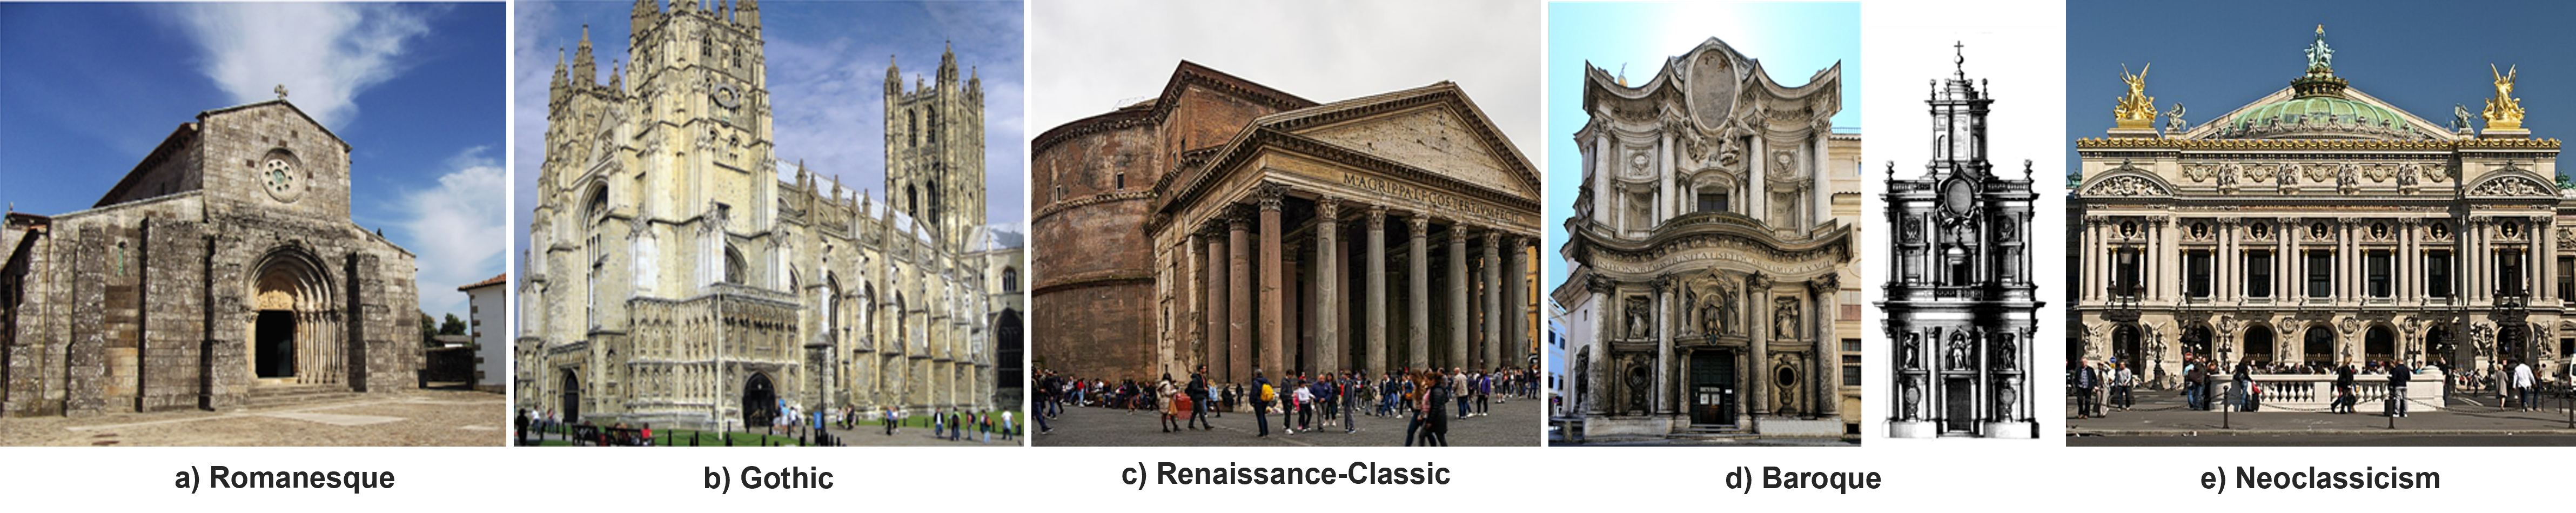
\includegraphics[width= \linewidth]{Images/OldTimeline}
                        \captionof{figure}{Early timeline. Sequential representation of architectural styles illustrating the shift between complexity and simplicity. From left to right: Romanesque[a] with its solid and massive structure; Gothic[b] featuring verticality and lightness; Classicism[c] characterized by geometrical clarity and order; Baroque[d] with dynamic shapes and rich decorations; followed by the restrained and symmetrical formality of Neo-classicism[e]. (\textit{Images edited from source})}
                        \label{fig:Oldtimeline}
            \end{minipage}
            \\
            %Middle cell
            %Middle timeline
            \begin{minipage}{\textwidth}
                \centering
                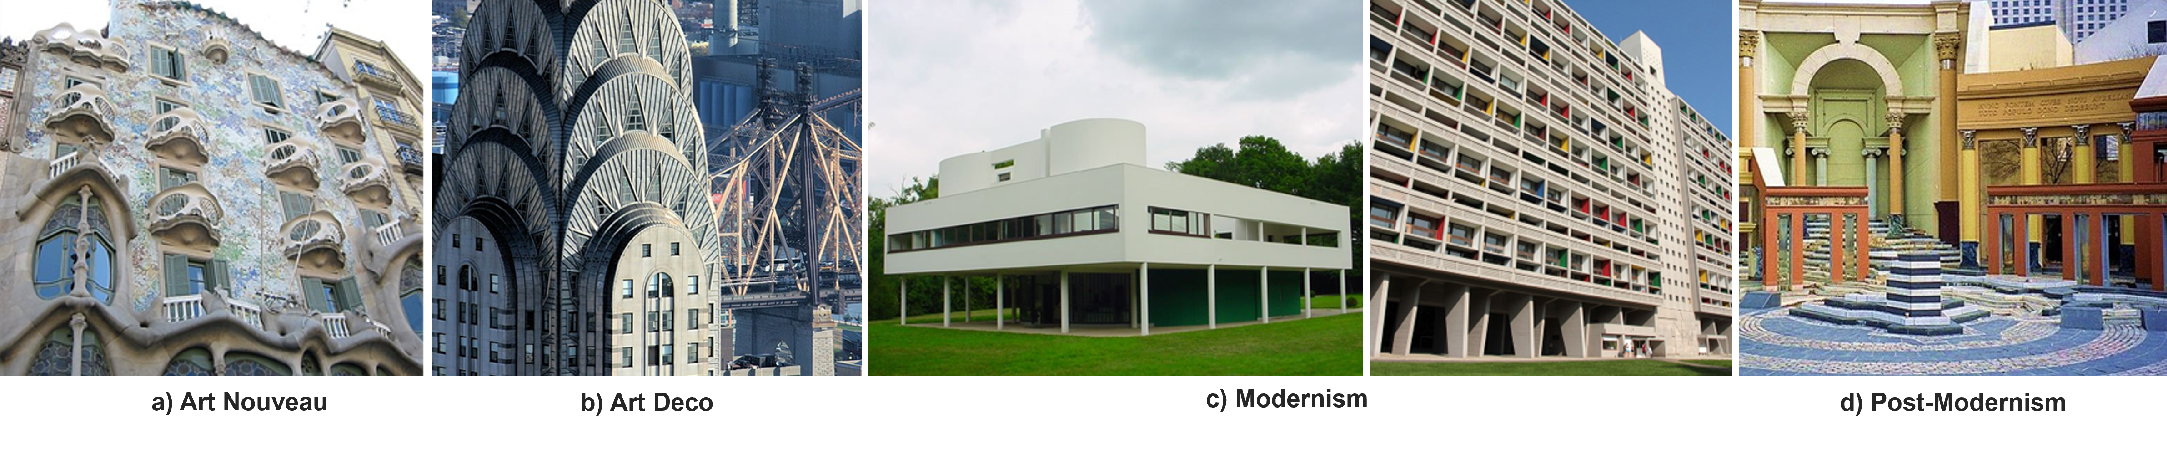
\includegraphics[width= \linewidth]{Images/MiddleTimeline}
                        \captionof{figure}{Transitional timeline. Sequential representation of architectural styles illustrating the shift between complexity and simplicity. From left to right: Art Nouveau[a] with its fluid lines and natural forms; Art Deco[b], marked by bold geometry and opulence; Modernism's[c] pursuit of stripped-back functionality; culminating in Postmodernism's[d] revival of historical styles and complexity (\textit{Images edited from source})}
                        \label{fig:Middletimeline}
            \end{minipage}
            \\
            %bottom Cell
            %Contemporary timeline
            \begin{minipage}{\textwidth}
                \centering
                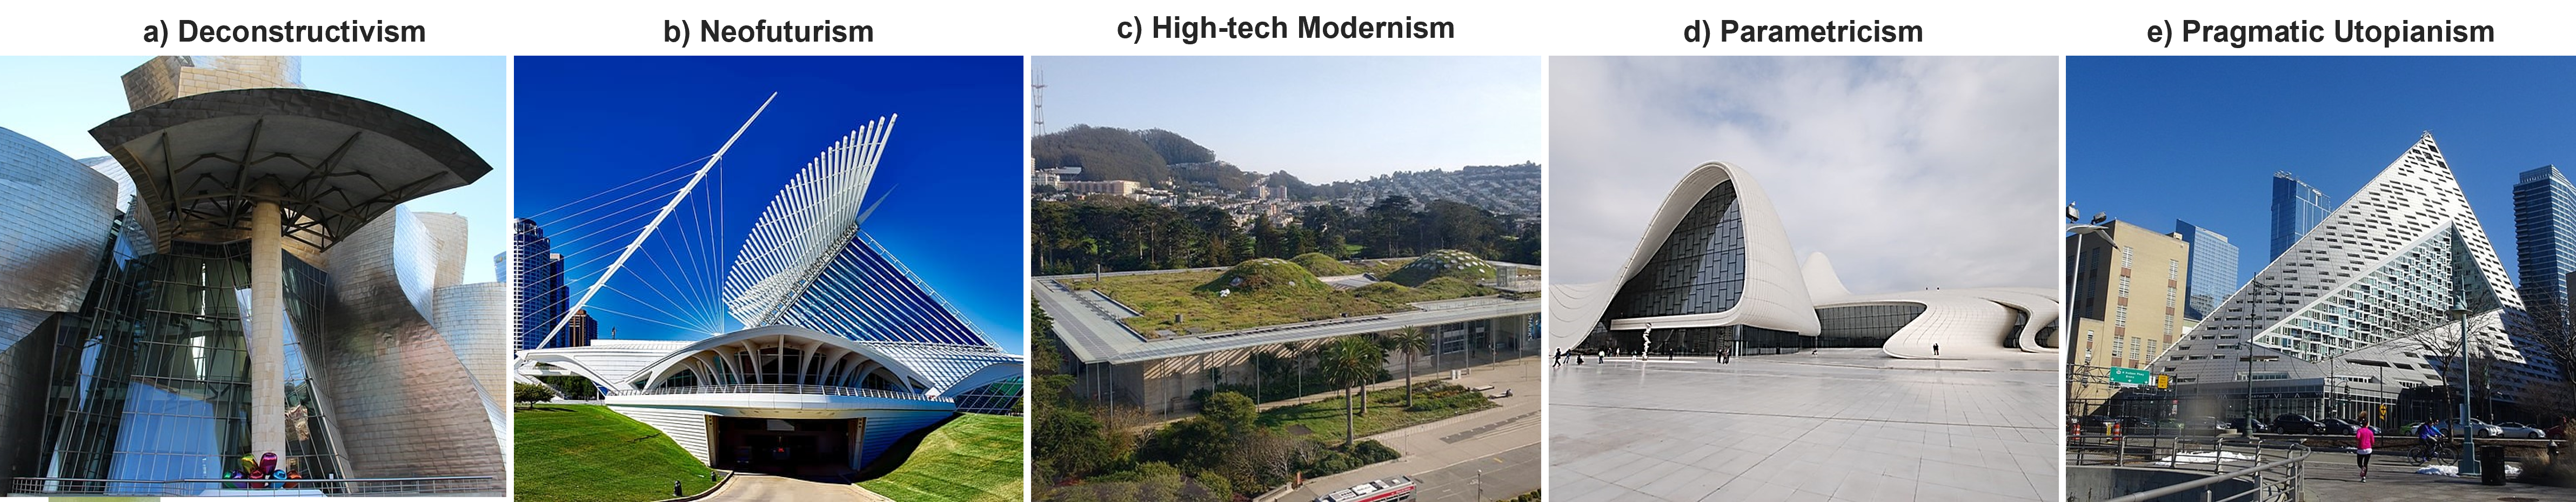
\includegraphics[width= \linewidth]{Images/contemporaryTimeline}
                        \captionof{figure}{Contemporary timeline. Sequential representation of architectural styles illustrating the shift between complexity and simplicity. Era of exploration and innovation. From left to right: Deconstructivism[a], characterized by fragmentation and non-linear design; Neofuturism[b], capturing movement and technology-infused aesthetics; High-tech modernism[c], focusing on visible structural elements and technological expression; Parametricism[d], with its algorithm-based complex forms; and Pragmatic utopianism[e], blending idealistic designs with practical applications (\textit{Images edited from source})}
                        \label{fig:contemporarytimeline}
            \end{minipage}
        \end{tabular}
    \end{table*}


\section{Literature review}
\label{sec:LiteratureReview}
%% Research Background

%% A Theory section should extend, not repeat, the background to the article already dealt with in the Introduction and lay the foundation for further work. In contrast, a Calculation section represents a practical development from a theoretical basis.

%A theoretical framework is a foundational review of existing theories that serves as a roadmap for developing the arguments you will use in your own work.

%=============================================================================
%Outline.
%1. Introduction
%2. The importance of facade in a building.
%3. A brief analysis of architecture styles and the shift from Images and simplicity
%3. A reflexion into digital fabrication techniques specially parametric design.
%4. The principle of data driven design.
%5. An analysis into mixed reality and the advantages of introducing this  into the design review.
%=============================================================================

%///////////////////////////////////////////////////////////////
%% refined outline of theory framework

%% Introduction

%!Concise intro

This section delves into the multifaceted nature of architectural complexity, examining its historical evolution and the theoretical foundations that underpin contemporary architectural practices.
It aims to provide a comprehensive understanding of how complexity influences both design practices and user experiences.
The literature review is organized into two key themes:

\begin{itemize}
    \item \textit{Evolution of Architectural Styles:} focusing on the historical transitions between simplicity and complexity in architecture, highlighting significant shifts across different periods.
    \item \textit{Theoretical Foundations of Architectural Complexity:} exploring foundational theories and previous research surrounding complexity in architecture, offering insights into how these theories inform current design practices.
\end{itemize}

\added{By linking historical analysis, and complexity theories with user perception studies, this review provides a framework for understanding how past architectural trends in complexity influence modern user preferences, allowing us to explore whether contemporary design trends align with these historical patterns.}
These insights are crucial for validating the CICA findings by comparing empirical data with theoretical perspectives on architectural evolution, thereby confirming observed patterns of simplicity and complexity.



    %Historical Context
\subsection{Evolution of Architectural Styles: Oscillations Between Simplicity and Complexity}
\label{subsec:TimelineArchitectureStyles}

Architecture stands as a unique art form, transforming the ordinary into the extraordinary while fulfilling functional purposes~\cite{Jiang2023}.
Its evolution is marked by a dynamic interplay between simplicity and complexity, reflecting societal values and technological advancements~\cite{Economakis2023}.
From early architectural styles like Romanesque, characterized by robust and simplistic forms, to the Gothic period with its intricate, skyward designs~\cite{Stacbond2020}, architecture has oscillated between simplicity and complexity (see Figure~\ref{fig:Oldtimeline} a,b).

The Renaissance heralded a revival of Greek and Roman ideals with a focus on symmetry, followed by the Baroque's lavish ornamentation in the 16th century~\cite{Economakis2023} (see Figure~\ref{fig:Oldtimeline} c,d).
The Neoclassical style, dominant in the 18th and 19th centuries, emphasized symmetry and classical principles while integrating new technologies like reinforced concrete~\cite{Economakis2023} (see Figure~\ref{fig:Oldtimeline} e).
Art Nouveau and Art Deco, emerging in the late 19th and early 20th centuries, celebrated nature and technological advancements, marking a departure from Neoclassical restraint~\cite{Salas2018, Arora2023} (see Figure~\ref{fig:Middletimeline} a, b).

The 20th century saw the rise of Modern Architecture, which advocated for `form follows function' and minimal ornamentation, a significant departure from previous ornate designs~\cite{Leach2016}.
Figures like Adolf Loos and Le Corbusier championed minimalism and functionality, influencing a generation of architects to prioritize structural honesty and simplicity~\cite{Saglam2014}.
However, this movement often led to uniform urban landscapes that lacked the cultural richness and diversity of their predecessors (see Figure~\ref{fig:Middletimeline} c).

In response to Modernism's perceived limitations, the late 1960s saw the emergence of Postmodernism, spearheaded by thinkers like Robert Venturi.
Postmodernism critiqued the minimalist aesthetic and reintroduced complexity, ornament, and form into architectural design, advocating for buildings that engage more deeply with their cultural and historical contexts~\cite{Venturi1972} (see Figure~\ref{fig:Middletimeline} d).

The late 20th and early 21st centuries have seen a resurgence in creativity and expression, with architects utilizing digital technologies to explore new realms of complexity and ornamentation~\cite{Burlando2019} (see Figure~\ref{fig:contemporarytimeline}).
The fusion of digital and physical design processes signals a shift towards the democratization of complex, parametric designs, indicative of a contemporary period that values ornamentation, functionality, and human comfort~\cite{Schwab2016}.
This evolving trajectory of architecture suggests a future where design is deeply intertwined with societal values and technological possibilities.

Facades and ornamentation, in this context, become critical in conveying these narratives, bridging the gap between the aesthetic and the symbolic, and establishing the interface between buildings and their environments, influencing comfort and energy efficiency while reflecting the building's identity~\cite{Kamal2020}.
The evolution of facade design and ornamentation mirrors societal transformations, technological progress, and shifts in artistic sensibilities, each impacting how communities relate to their built environment.

In conclusion, the historical context of architectural complexity reveals a rich tapestry of styles and philosophies, from ancient grandiosity to modern minimalism and contemporary innovation.
These shifts reflect the ongoing dialogue between simplicity and complexity, tradition and innovation, and functionality and aesthetics, shaping the built environment in ways that are both imaginative and responsive to societal needs.


\subsection{Theoretical Foundations of Architectural Complexity}
\label{subsec:ComplexityStudies}

Previous research has extensively explored the impact of complexity in architectural design, showing that elements such as chaotic patterns and fractal geometry significantly influence user perceptions and aesthetic preferences~\cite{Bies2016}.
Contemporary studies suggest that balanced complexity can create environments that are both stimulating and comfortable~\cite{Redies2015}.
However, the architectural field has yet to fully develop frameworks that leverage these principles for practical design applications, particularly with modern technological advancements.

A foundational theoretical contribution to understanding architectural complexity is George David Birkhoff's theory of aesthetic measure, introduced in 1933.
Birkhoff proposed that aesthetic value could be quantified through a ratio of order to complexity, expressed as M = O/C (where M is the aesthetic measure, O is order, and C is complexity)\cite{Douchova2016}.
This theory provided a framework for evaluating the aesthetic appeal of architectural forms based on their structural and decorative elements.
Despite challenges to the validity of Birkhoff's method for penalizing complexity, the concepts of order and complexity, along with objective quantification methods, remain significant in aesthetic evaluation functions\cite{Javaheri2016}.
This balance is central to contemporary efforts to integrate complexity into architectural design, enhancing both user satisfaction and sustainability.

Another significant theoretical framework is Alexander et al.~concept of `pattern language,' introduced in the 1970s~\cite{Alexander1977}.
Alexander et al.~emphasized the importance of recurring design patterns that resonate fundamentally with human users.
is theory suggests that certain patterns, when combined effectively, create environments that feel harmonious and alive, aligning with biophilic design principles that seek to connect architecture with natural elements to enhance human well-being~\cite{Downton2017}.

Browning et al.~(2014) contribute to this discussion by emphasizing the importance of balancing complexity and order in architectural design.
Their research highlights that visually engaging and information-rich spaces should strike a balance between being overly simplistic and overwhelmingly complex.
They draw from studies on fractal geometries found in nature, art, and architecture, suggesting that certain fractal dimensions (D=1.3-1.8) are preferred for their aesthetic and stress-reducing qualities~\cite{Browning2014}.
Fractal designs with three iterations are particularly effective in conveying a sense of order and intrigue.
These principles can be applied to various architectural elements to promote visually stimulating environments that support psychological and cognitive well-being.
However, they caution against the extremes of non-fractal or overly complex designs, which can induce stress or discomfort.
The goal is to integrate fractal geometries and hierarchies into design to create environments that are both engaging and restorative~\cite{Browning2014}.

A more recent method by Lee et al.~(2023) uses fractal dimension analysis to measure the visual complexity of architectural facades, which is crucial for assessing aesthetic character and predicting attractiveness.
They utilized the differential box counting method, which is better suited for handling greyscale images, to calculate fractal dimensions based on grey-level variations.
These fractal dimension values are then used to predict human visual preferences, providing a reliable measure of visual complexity in architectural design~\cite{Lee2023}.
Lee et al.~concluded that computational measures of visual complexity (fractal dimensions) and attractive strength (visual attention simulation) can effectively quantify the visual attractiveness of architectural facades.
Their findings indicate that these measures can distinguish different architectural styles, despite some limitations.
Importantly, they found that visual complexity (D) and attractive strength (S) are not mathematically correlated, suggesting that engagement and appeal may be independent qualities.
The proposed model for predicting visual attractiveness, A = D × S, will require further validation.
This study highlights the significant influence of visual attractiveness on perceptions of architecture and the need to evaluate these attributes during the design process~\cite{Lee2023}.

Contemporary research continues to build on these theoretical foundations, exploring how advanced technologies can be used to create complex designs that are both aesthetically pleasing and functionally effective.
The integration of digital tools such as BIM and computational design methods has enabled architects to push the boundaries of complexity, creating structures that are not only visually striking but also optimized for performance and sustainability, offering visually stimulating and experientially rich environments~\cite{Leach2016}~(Figure~\ref{fig:contemporarytimeline}).

In summary, the evolution of architectural complexity reflects an ongoing interplay between cultural, technological, and theoretical influences.
From ancient grandiosity to modern minimalism and contemporary innovation, architects have continually sought to balance order and complexity to create meaningful and engaging built environments.
Theoretical frameworks such as Birkhoff's aesthetic measure, Alexander's pattern language, and Lee et al.'s fractal dimension analysis provide valuable insights into harnessing complexity to enhance architectural design, offering a foundation for future explorations in this dynamic field.

Despite significant advancements in understanding architectural complexity and its impact on user perceptions, there remains a notable gap in the integration of theoretical insights with practical applications in the context of modern technological advancements.
Current methodologies often lack the ability to provide real-time, interactive evaluations of facade complexity, limiting their applicability in dynamic design environments.
My research aims to bridge this gap by developing a comprehensive system that combines immersive VR experiences with CV algorithms embedded in the CICA system.
This approach allows for the quantification of facade complexity in a way that is both interactive and responsive to user feedback, providing a practical tool for architects to optimize design complexity while considering aesthetic and functional aspects.
By incorporating advanced digital tools and empirical data, this research seeks to enhance the understanding of how complexity can be effectively managed and utilized in contemporary architectural practices.



    %\subsection{The Architectural Journey: Oscillations Between Simplicity and Complexity}
    %\label{subsec:TimelineArchitectureStyles}
    %\input{Text/TheoryHistoryArchStyles}

    %\subsection{Evolution and Theoretical Foundations of Architectural Complexity}
    %\label{subsec:ComplexityStudies}
    %%Historical Context
\subsection{Evolution of Architectural Styles: Oscillations Between Simplicity and Complexity}
\label{subsec:TimelineArchitectureStyles}

Architecture stands as a unique art form, transforming the ordinary into the extraordinary while fulfilling functional purposes~\cite{Jiang2023}.
Its evolution is marked by a dynamic interplay between simplicity and complexity, reflecting societal values and technological advancements~\cite{Economakis2023}.
From early architectural styles like Romanesque, characterized by robust and simplistic forms, to the Gothic period with its intricate, skyward designs~\cite{Stacbond2020}, architecture has oscillated between simplicity and complexity (see Figure~\ref{fig:Oldtimeline} a,b).

The Renaissance heralded a revival of Greek and Roman ideals with a focus on symmetry, followed by the Baroque's lavish ornamentation in the 16th century~\cite{Economakis2023} (see Figure~\ref{fig:Oldtimeline} c,d).
The Neoclassical style, dominant in the 18th and 19th centuries, emphasized symmetry and classical principles while integrating new technologies like reinforced concrete~\cite{Economakis2023} (see Figure~\ref{fig:Oldtimeline} e).
Art Nouveau and Art Deco, emerging in the late 19th and early 20th centuries, celebrated nature and technological advancements, marking a departure from Neoclassical restraint~\cite{Salas2018, Arora2023} (see Figure~\ref{fig:Middletimeline} a, b).

The 20th century saw the rise of Modern Architecture, which advocated for `form follows function' and minimal ornamentation, a significant departure from previous ornate designs~\cite{Leach2016}.
Figures like Adolf Loos and Le Corbusier championed minimalism and functionality, influencing a generation of architects to prioritize structural honesty and simplicity~\cite{Saglam2014}.
However, this movement often led to uniform urban landscapes that lacked the cultural richness and diversity of their predecessors (see Figure~\ref{fig:Middletimeline} c).

In response to Modernism's perceived limitations, the late 1960s saw the emergence of Postmodernism, spearheaded by thinkers like Robert Venturi.
Postmodernism critiqued the minimalist aesthetic and reintroduced complexity, ornament, and form into architectural design, advocating for buildings that engage more deeply with their cultural and historical contexts~\cite{Venturi1972} (see Figure~\ref{fig:Middletimeline} d).

The late 20th and early 21st centuries have seen a resurgence in creativity and expression, with architects utilizing digital technologies to explore new realms of complexity and ornamentation~\cite{Burlando2019} (see Figure~\ref{fig:contemporarytimeline}).
The fusion of digital and physical design processes signals a shift towards the democratization of complex, parametric designs, indicative of a contemporary period that values ornamentation, functionality, and human comfort~\cite{Schwab2016}.
This evolving trajectory of architecture suggests a future where design is deeply intertwined with societal values and technological possibilities.

Facades and ornamentation, in this context, become critical in conveying these narratives, bridging the gap between the aesthetic and the symbolic, and establishing the interface between buildings and their environments, influencing comfort and energy efficiency while reflecting the building's identity~\cite{Kamal2020}.
The evolution of facade design and ornamentation mirrors societal transformations, technological progress, and shifts in artistic sensibilities, each impacting how communities relate to their built environment.

In conclusion, the historical context of architectural complexity reveals a rich tapestry of styles and philosophies, from ancient grandiosity to modern minimalism and contemporary innovation.
These shifts reflect the ongoing dialogue between simplicity and complexity, tradition and innovation, and functionality and aesthetics, shaping the built environment in ways that are both imaginative and responsive to societal needs.


\subsection{Theoretical Foundations of Architectural Complexity}
\label{subsec:ComplexityStudies}

Previous research has extensively explored the impact of complexity in architectural design, showing that elements such as chaotic patterns and fractal geometry significantly influence user perceptions and aesthetic preferences~\cite{Bies2016}.
Contemporary studies suggest that balanced complexity can create environments that are both stimulating and comfortable~\cite{Redies2015}.
However, the architectural field has yet to fully develop frameworks that leverage these principles for practical design applications, particularly with modern technological advancements.

A foundational theoretical contribution to understanding architectural complexity is George David Birkhoff's theory of aesthetic measure, introduced in 1933.
Birkhoff proposed that aesthetic value could be quantified through a ratio of order to complexity, expressed as M = O/C (where M is the aesthetic measure, O is order, and C is complexity)\cite{Douchova2016}.
This theory provided a framework for evaluating the aesthetic appeal of architectural forms based on their structural and decorative elements.
Despite challenges to the validity of Birkhoff's method for penalizing complexity, the concepts of order and complexity, along with objective quantification methods, remain significant in aesthetic evaluation functions\cite{Javaheri2016}.
This balance is central to contemporary efforts to integrate complexity into architectural design, enhancing both user satisfaction and sustainability.

Another significant theoretical framework is Alexander et al.~concept of `pattern language,' introduced in the 1970s~\cite{Alexander1977}.
Alexander et al.~emphasized the importance of recurring design patterns that resonate fundamentally with human users.
is theory suggests that certain patterns, when combined effectively, create environments that feel harmonious and alive, aligning with biophilic design principles that seek to connect architecture with natural elements to enhance human well-being~\cite{Downton2017}.

Browning et al.~(2014) contribute to this discussion by emphasizing the importance of balancing complexity and order in architectural design.
Their research highlights that visually engaging and information-rich spaces should strike a balance between being overly simplistic and overwhelmingly complex.
They draw from studies on fractal geometries found in nature, art, and architecture, suggesting that certain fractal dimensions (D=1.3-1.8) are preferred for their aesthetic and stress-reducing qualities~\cite{Browning2014}.
Fractal designs with three iterations are particularly effective in conveying a sense of order and intrigue.
These principles can be applied to various architectural elements to promote visually stimulating environments that support psychological and cognitive well-being.
However, they caution against the extremes of non-fractal or overly complex designs, which can induce stress or discomfort.
The goal is to integrate fractal geometries and hierarchies into design to create environments that are both engaging and restorative~\cite{Browning2014}.

A more recent method by Lee et al.~(2023) uses fractal dimension analysis to measure the visual complexity of architectural facades, which is crucial for assessing aesthetic character and predicting attractiveness.
They utilized the differential box counting method, which is better suited for handling greyscale images, to calculate fractal dimensions based on grey-level variations.
These fractal dimension values are then used to predict human visual preferences, providing a reliable measure of visual complexity in architectural design~\cite{Lee2023}.
Lee et al.~concluded that computational measures of visual complexity (fractal dimensions) and attractive strength (visual attention simulation) can effectively quantify the visual attractiveness of architectural facades.
Their findings indicate that these measures can distinguish different architectural styles, despite some limitations.
Importantly, they found that visual complexity (D) and attractive strength (S) are not mathematically correlated, suggesting that engagement and appeal may be independent qualities.
The proposed model for predicting visual attractiveness, A = D × S, will require further validation.
This study highlights the significant influence of visual attractiveness on perceptions of architecture and the need to evaluate these attributes during the design process~\cite{Lee2023}.

Contemporary research continues to build on these theoretical foundations, exploring how advanced technologies can be used to create complex designs that are both aesthetically pleasing and functionally effective.
The integration of digital tools such as BIM and computational design methods has enabled architects to push the boundaries of complexity, creating structures that are not only visually striking but also optimized for performance and sustainability, offering visually stimulating and experientially rich environments~\cite{Leach2016}~(Figure~\ref{fig:contemporarytimeline}).

In summary, the evolution of architectural complexity reflects an ongoing interplay between cultural, technological, and theoretical influences.
From ancient grandiosity to modern minimalism and contemporary innovation, architects have continually sought to balance order and complexity to create meaningful and engaging built environments.
Theoretical frameworks such as Birkhoff's aesthetic measure, Alexander's pattern language, and Lee et al.'s fractal dimension analysis provide valuable insights into harnessing complexity to enhance architectural design, offering a foundation for future explorations in this dynamic field.

Despite significant advancements in understanding architectural complexity and its impact on user perceptions, there remains a notable gap in the integration of theoretical insights with practical applications in the context of modern technological advancements.
Current methodologies often lack the ability to provide real-time, interactive evaluations of facade complexity, limiting their applicability in dynamic design environments.
My research aims to bridge this gap by developing a comprehensive system that combines immersive VR experiences with CV algorithms embedded in the CICA system.
This approach allows for the quantification of facade complexity in a way that is both interactive and responsive to user feedback, providing a practical tool for architects to optimize design complexity while considering aesthetic and functional aspects.
By incorporating advanced digital tools and empirical data, this research seeks to enhance the understanding of how complexity can be effectively managed and utilized in contemporary architectural practices.



    %\subsection{Cultural Significance of Facades and Ornament}
    %\label{subsec:FacadeandOrnament}
    %
%!subsection{Cultural Significance of Facades and Ornament}
%!\label{subsec: FacadeandOrnament}

%!==========================
%Delve deeper into how facades reflect cultural values, societal norms, and historical contexts. Explore how different societies and civilizations have expressed their identity through architectural ornamentation and symbolism.
%!==========================

%!Concise version
Architecture, transcending its primary role of providing shelter, serves as a canvas reflecting the cultural, historical, and societal narratives of its time.
Facades and ornamentation, in this context, become critical in conveying these narratives, bridging the gap between the aesthetic and the symbolic, and establishing the interface between buildings and their environments, influencing comfort and energy efficiency, while reflecting the building's identity\cite{Kamal2020}.

While the previous section traced the oscillations between simplicity and complexity in architectural styles to establish a foundation for the notion that contemporary architecture is gravitating towards a renaissance of complexity, here we explore the underlying cultural currents that influenced these shifts.
The evolution of facade design and ornamentation mirrors societal transformations, technological progress, and shifts in artistic sensibilities, each impacting how communities relate to their built environment.

%Facades according to Vitruvius

Vitruvius, in his 1st-century BCE work `De Architectura', outlined principles for architecture that emphasize structural soundness, functionality, and beauty\cite{Ostwald2023}.
He advocated for harmony and balance in design, using the principle of `Decor' to guide appropriate articulation that respects religious, natural, and social conventions\cite{Lefas2000}.
Vitruvius's principles, dormant for centuries, found renewed interest during the Renaissance and continued through the Neoclassical and Ecole des Beaux-Arts styles\cite{Wikipedia2023}.
This revival reinforced the classical architectural aesthetics rooted in order and rationality (Figure\ref{fig:Oldtimeline} c,e).
The principles of Vitruvius, emphasizing a balance of structural integrity, functionality, and aesthetics, have had a lasting impact, shaping the trajectory of architectural design and ornamentation throughout history.

%facade according to bernini and borromini

Moving beyond the Renaissance era and into the Baroque style, a significant shift in the perception of facades and ornamentation occurs.
Francesco Borromini, a prominent Italian architect of the Baroque period, emerges as a key figure in this context.
Borromini's architectural philosophy revolved around the facade as a reflection of a building's interior.
He viewed the facade not just as an ornamental feature but as a visual representation of the internal spaces and functions\cite{Benjamin2006}.
Borromini's designs often featured elaborate geometric patterns, curved forms, and sculptural elements, integrating the facade with the building's spatial organization and internal arrangement.
This approach is exemplified in his works, such as the San Carlo alle Quattro Fontane Church in Rome (Figure\ref{fig:Oldtimeline} d).

Borromini's perspective on facades transcended surface aesthetics.
He believed facades should express the building's deeper design and purpose, embodying an expressive display of interiority and an invitation for an external reading\cite{Biglieri2004}.
This philosophy underscores the integral role of facades in the overall architectural composition during the Baroque period.

% context on neo classic, art nouveau and art deco

In tracing the evolution of facades and ornamentation, it's important to recognize the architectural periods that significantly influenced the field, bridging the gap between the Baroque era and the transformative epoch of Modernism.
Notable styles in this transition include Neo-Classicism, Art Nouveau, and Art Deco.

Neo-Classical architecture (late 18th to early 19th centuries) revived Vitruvian principles and Palladian ideals.
It emphasized formal elegance and symmetry, often featuring facades with balanced proportions and columns (Figure\ref{fig:Oldtimeline} e).
Art Nouveau (late 19th to early 20th centuries), led by architects like Gaudi, introduced organic forms into facade design.
Gaudi's work, such as Casa Batlló, utilized flowing lines and natural motifs\cite{Nasir2022} (Figure\ref{fig:Middletimeline} a).
Art Deco (1920s to early 1930s) merged luxury and technological progress, characterized by geometric shapes, high-contrast colors, and metallic surfaces, as seen in the Chrysler Building\cite{Kotb2014} (Figure\ref{fig:Middletimeline} b).
While these styles contributed to the diversity of architectural aesthetics, they did not initiate the profound paradigm shifts that Modernism would later bring.
With this context, we now turn to the significant impact of the Modernist movement on architectural philosophy.

% Modernism and facade according to Le Corbusier

The transition into the 20th century's Modernist style marked a significant shift in the approach to facades and ornamentation.
As discussed in the previous section, this era, saw a move away from traditional ornamental design.

Loos, in his 1908 article `Ornament and Crime', a prominent figure on this movement, championed functional design and critiqued conventional ornamentation\cite{Saglam2014}.
Le Corbusier, a key Modernist architect, further revolutionized facade design.
His work, particularly `Towards a New Architecture'\cite{Studio2a2023} and `The Five Points of a New Architecture', emphasized minimalism and utility.
He advocated for facades that reflect a building's purpose and the well-being of its occupants, adhering to his human-centric design philosophy\cite{Virseda2021}.

Le Corbusier's concept of `Free design of the facade'\cite{Corbusier1986} allowed for innovative use of materials and structural elements to create functional ornamentation.
His designs often featured large windows, sunshades, and brise-soleil, prioritizing light, ventilation, and climate control while maintaining aesthetic integrity (Figure\ref{fig:Middletimeline} c).
Thus, Le Corbusier's views on facades represent a blend of clarity, rationality, and harmonious integration, rejecting excess adornment while celebrating structural innovation and technological advancements.

% Postmodernism and facade according to Venturi

Despite the innovative drive of Modernism, its utopian vision often fell short in materializing human-centric environments, leading to spaces that felt monotonous and detached from cultural contexts.
This paved the way for Robert Venturi's critical perspective on Modernism and his pioneering role in the Postmodernism movement.

Venturi, in his seminal works like `Complexity and Contradiction in Architecture' and `Learning From Las Vegas', challenged the Modernist ideals, advocating for architecture that embraced complexity, contradiction, and meaningful ornamentation \cite{Venturi1977}.
He criticized the Modernist approach for its oversimplification and lack of symbolic expression, arguing for an architecture that responds to cultural context and human experience (Figure\ref{fig:Middletimeline} d).



Venturi's approach to facades and ornamentation incorporated diverse elements, historical references, and bright colors, challenging the minimalist ethos of Modernism.
He believed in the richness of symbolism and the importance of integrating elements from historical precedents into contemporary design\cite{Venturi1971}.
His famous dictum, `Less is a bore', encapsulated his critique of Modernist minimalism and his advocacy for thoughtful ornamentation.

Venturi's vision encouraged the use of facades as mediums to communicate various meanings, evoke emotions, and respond to their cultural and contextual surroundings.
His influence in Postmodernism expanded architectural horizons, urging architects to embrace diversity, historical resonance, and meaningful expression in their designs\cite{Lutolli2020, Stamp2016}

%Contemporary styles

Following Postmodernism, contemporary architecture witnessed a shift towards more dynamic and diverse styles, including Deconstructivism, Neofuturism, High-tech modernism, Parametricism, and Pragmatic utopianism.
These styles collectively signify a move towards complexity in facade design and ornamentation, influenced by advancements in technology and a focus on sustainability.

Deconstructivism, characterized by fragmentation and non-rectilinear shapes, was exemplified by architects like Frank Gehry, who integrated unconventional forms into their designs (Figure\ref{fig:contemporarytimeline} \textit{a}).
Neofuturism, represented by architects like Santiago Calatrava, embraced a futuristic aesthetic with dynamic, flowing forms (Figure\ref{fig:contemporarytimeline} \textit{b}).
High-tech modernism, or structural expressionism, focused on showcasing technological components and advanced materials, as seen in works by Renzo Piano and Norman Foster (Figure\ref{fig:contemporarytimeline} \textit{c}).
Parametricism, often associated with Zaha Hadid, utilized computational design to create intricate geometries and dynamic structures (Figure\ref{fig:contemporarytimeline} \textit{d}).
Pragmatic utopianism, exemplified by Bjarke Ingels, combined ambitious visions with practical solutions, focusing on functionality, sustainability, and meaningful ornamentation (Figure\ref{fig:contemporarytimeline} \textit{e}).
These styles reflect the architectural evolution from the late 20th century into the 21st, showcasing a variety of approaches to facades and ornamentation that blend tradition with innovation.


%conclusion
In conclusion, the journey through the evolution of facade and ornament theory reveals a rich tapestry of architectural ingenuity, shaped by cultural, technological, and artistic influences.
From the foundational principles of Vitruvius to the ornate expressions of the Baroque period, the functional minimalism of Modernism, and the eclectic approaches of Postmodernism, each era has contributed distinct perspectives on the relationship between a building's exterior and its intrinsic character.

Contemporary styles like Deconstructivism, Neofuturism, High-tech Modernism, Parametricism, and Pragmatic Utopianism (see Figure\ref{fig:contemporarytimeline}) further demonstrate the diversity and dynamism in current architectural practice.
These styles collectively underscore an ongoing dialogue between simplicity and complexity, tradition and innovation, functionality and aesthetics.

As we look towards the future, the continued evolution of facade and ornament theory will undoubtedly be influenced by emerging technologies, sustainability concerns, and the ever-changing needs of human societies, shaping the built environment in ways that are both imaginative and responsive to the world around us.

The cultural significance of facades extends beyond aesthetic appeal, contributing to a community's sense of identity and continuity.
As we look to the future, the challenge and opportunity lie in harnessing emerging technologies to create architecture that resonates with societal values and cultural diversity, thereby enriching the urban landscape.






    %\subsection{Digital fabrication and Environmental Sustainability}
    %\label{subsec:DigitalFabricationAndEnvSustainability}
    %
%!\subsection{Digital fabrication and Environmental Sustainability}
%!\label{subsec:DigitalFabricationAndEnvSustainability}

%!==========================
%8. **Environmental Sustainability:** Investigate how the integration of complex facades and digital fabrication aligns with contemporary sustainability principles. Examine how parametric design and data-driven approaches can enhance energy efficiency, reduce material waste, and contribute to sustainable construction practices.
%!==========================
To be revised ...
%!original

%Digital fabrication technologies, meanwhile, are interacting with the biological world on a daily basis.
%Engineers, designers, and architects are combining computational design, additive manufacturing, materials engineering, and synthetic biology to pioneer a symbiosis between microorganisms, our bodies, the products we consume, and even the buildings we inhabit\cite{Schwab2016}.







    %!% Figures Methodology intro
    %% Methodology Flowchart
    \begin{figure*}[!htb]
        \centering
        \includegraphics[width=\linewidth]{Images/MethodologyFlowchart}~\caption{Methodology Flowchart illustrating the sequential steps of this study's approach framework designed to assess the qunatification of complexity in building design and the perception of occupants in complex environemnts. Higlighting the usage of the CICA system (element 2) (detailed in Section~\ref{subsubsec:CICAsystem}) in the Complexity Analysis System development (detailed in Section\ref{subsec:ComplexitySystemDevelopment}), and the transition to `Experiment Execution' (element 4) (described in Section\ref{subsec:Experiment_execution}), culminating in the post-experiment data analysis and results phase (element 5) (described in Section\ref{subsec:Data_analysis}).}
          \label{fig:MethodologyFlowchart}
    \end{figure*}

    %% CICA Flowchart
    %\begin{table*}[htb]
%            \centering
%            \small
%            \begin{tabular}{c}
%                %Top cell with one figure
%                %Figure Computational Image Compexity Analysis (CICA) System flowchart
%                \begin{minipage}{\textwidth}
%                    \centering
%                    \includegraphics[width= \linewidth]{Images/CICAFlowchart}
%                    \captionof{figure}{Flowchart illustrating the applications of CICA system (detailed in Section\ref{subsec:CICAsystem}), including its role in analyzing complexity scores for historical architectural styles (b) and 3D-modeled facades (a) designed with various degrees of complexity(presented in Section\ref{subsubsec:CICAfor3DmodeledFacades}).}
%                    \label{fig:CICAImageEvaluationFlowchart}
%                \end{minipage}
%            \end{tabular}
%            \end{table*}


\section{Methodology}
\label{sec:Methodology}
%%Methodology
%% methodology Intro
The methodology of this study, comprises three main components (as illustrated in  Figure~\ref{fig:MethodologyFlowchart}):
\begin{enumerate}
    \item \textit{Complexity Analysis System Development:}  Outlined in Section~\ref{subsec:ComplexitySystemDevelopment} and illustrated in Figure~\ref{fig:MethodologyFlowchart} (element 3.1), this component integrates the VR and CICA systems to create an immersive environment for evaluating facade complexities.
    \item \textit{Experiment Execution:} Detailed in Section~\ref{subsec:Experiment_execution} and illustrated in Figure~\ref{fig:MethodologyFlowchart} (element 3.2), involves the deployment of the VR component of the `Complexity Analysis' system in a controlled scenario to evaluate users' perception and response to different complexity levels in facade designs.
    \item \textit{Data Analysis and Validation:} Detailed in Section~\ref{subsec:Data_analysis} and illustrated in Figure~\ref{fig:MethodologyFlowchart} (element 3.3), this component analyzes the collected data to validate the VR system and CICA framework's effectiveness in measuring complexity and users' acceptance of building complexity.
\end{enumerate}

With the methodology outlined, we now move forward to a comprehensive breakdown of each component.


%\textbf{CICA system:} Detailed in Section~\ref{subsec:CICAsystem} and depicted as (3.1) in Figure~\ref{fig:MethodologyFlowchart}, involves developing a Python script using computer vision algorithms to process images and yield complexity scores, quantitatively gauging the intricacy of architectural designs.
%It supports theoretical analyses and provides a ranking framework for facade designs in the VR system.
%
%\textbf{VR System Development:}  Outlined in Section~\ref{subsec:VRsystemDevelopment} and represented as (3.2) in Figure~\ref{fig:MethodologyFlowchart}, this component focuses on creating an immersive experience where participants can explore and interact with a building's interior and exterior, manipulating facade designs with variable complexity levels and experiencing their impact.
%
%\textbf{Experiment Execution:} Detailed in Section~\ref{subsec:Experiment_execution} and illustrated as (3.3) in Figure~\ref{fig:MethodologyFlowchart}, following a similar approach to previous studies~\cite{Wolfartsberger2019}, this component outlines the method to evaluate users' acceptance of building complexity.
%It consists of three stages: a VR interaction stage, a screen-based stage, and a post-interaction survey.
%These stages allow for the collection of quantitative and qualitative data on participants' perceptions and responses to different complexity levels in facade designs.
%
%As illustrated in the methodology flowchart (Figure~\ref{fig:MethodologyFlowchart}), these components are combined to integrate computational analysis with immersive VR experiments, exploring user preferences in facade design and providing insights into architectural trends.
%
%With this methodology outlined, the following sections will now delve into a comprehensive breakdown of each component, highlighting their objectives, methodologies, and significance in achieving our research goals.


    %Figure Real vs 3d Model
    \begin{table*}[!htb]
    \centering
    \small
    \begin{tabular}{c}
        %Top cell with one figure
        %Figure Real vs 3d Model
        \begin{minipage}{\textwidth}
        \centering
        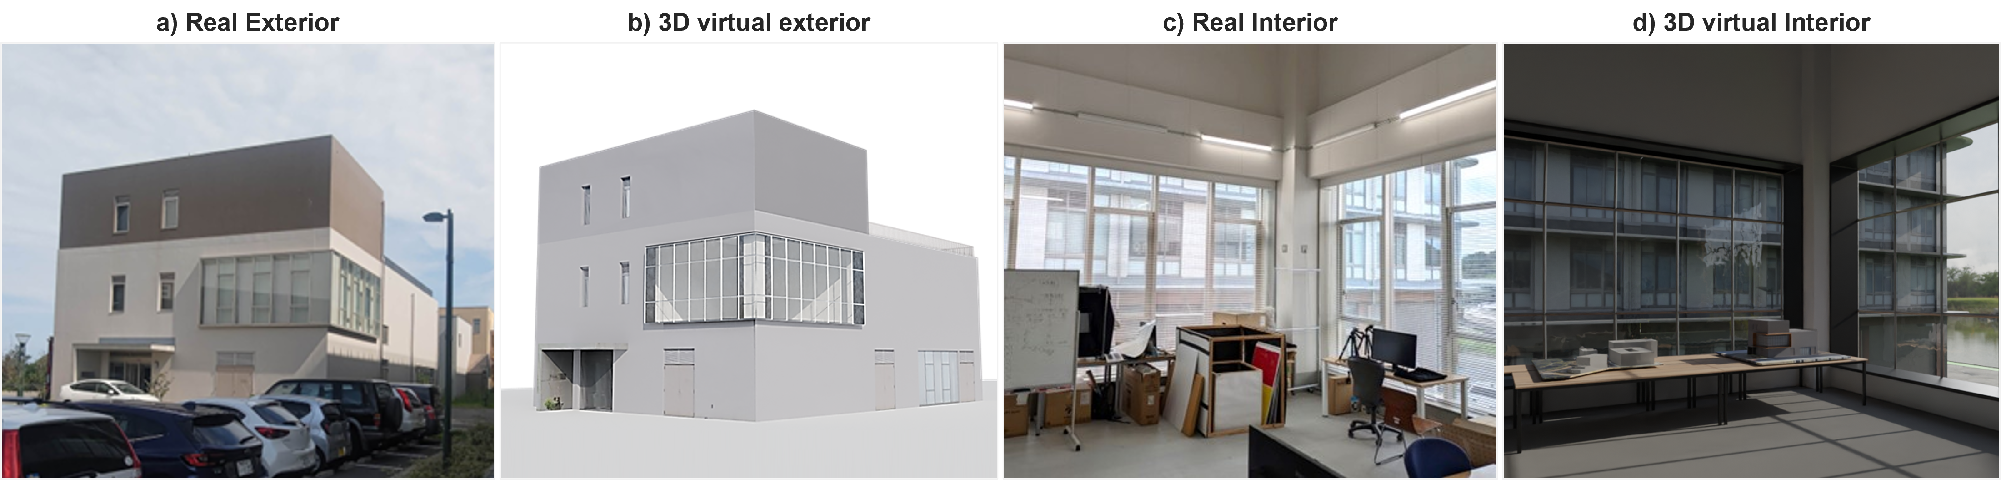
\includegraphics[width= \linewidth]{Images/Realvs3DmodelBlender}
                    \captionof{figure}{Comparison side by side of the actual Architectural Environment Building exterior (a) and interior (c) with its detailed 3D virtual clone counterpart (b, d) created for the VR experiment for Facade complexity Analysis, demonstrating the fidelity of the digital model in replicating architectural nuances.}
                    \label{fig:RealVs3dModel}
        \end{minipage}
        \\
        \\
        \\
        %Bottom cell
        %Table: Table: Pattern Variations sample 1, 7, 9
        \begin{minipage}{\textwidth}
            \centering
            \captionof{table}{Table of Facade Pattern Variations: This table presents samples of 3D-modeled building facades at levels 1, 7, and 9, showcasing the progression and differentiation within the ten levels of design variations as detailed in section~\ref{subsubsec:3DModeling}. The incremental complexity introduced at each selected level is highlighted across three distinct patterns. For a comprehensive record of all variations, refer to~\ref{sec:AnnexVariations}.}
            \label{tab:PatternsVariationsPart0}
            \begin{tabularx}
            {\textwidth}{p{3cm} >{\centering\arraybackslash}X >{\centering\arraybackslash}X >{\centering\arraybackslash}X }
        \toprule
        \multicolumn{4}{c}{\textbf{Progression of 3D-Modeled Facade Variations Across Patterns: A Comparative Analysis at Levels 1, 5, and 9}}\\
        \toprule
        \textit{Description} &
          \textit{Pattern 1} &
          \textit{Pattern 2} &
          \textit{Pattern 3} \\
        \midrule
        \text{Pattern Name} & Hishi Pattern & Tortoise shells & Asanoha Pattern\\

        \midrule
        \textit{Base Module} &  &  &
        \\
        {\includegraphics[width=1\linewidth]{Images/Base Module/Building}} &
          {\includegraphics[width=1\linewidth]{Images/Base Module/Pattern1}} &
          {\includegraphics[width=1\linewidth]{Images/Base Module/Pattern2}} &
          {\includegraphics[width=1\linewidth]{Images/Base Module/Pattern3}} \\
        \midrule

        \textit{Mesh complexity Level} &
          \textit{Pattern 1} &
          \textit{Pattern 2} &
          \textit{Pattern 3}\\

        \midrule
        \textit{Level 1} &  &  &
        \\
        {\includegraphics[width=1\linewidth]{Images/Wall 0/0001}} &
            {\includegraphics[width=1\linewidth]{Images/Pattern 1/0001}} &
          {\includegraphics[width=1\linewidth]{Images/Pattern 2/0001}} &
          {\includegraphics[width=1\linewidth]{Images/Pattern 3/0001}} \\
        \midrule
        \textit{Level 7} &  &  &
        \\
        {\includegraphics[width=1\linewidth]{Images/Wall 0/0007}} &
          {\includegraphics[width=1\linewidth]{Images/Pattern 1/0007}} &
          {\includegraphics[width=1\linewidth]{Images/Pattern 2/0007}} &
          {\includegraphics[width=1\linewidth]{Images/Pattern 3/0007}} \\
        \midrule
        \text{Level 9} &  &  &
        \\
        {\includegraphics[width=1\linewidth]{Images/Wall 0/0009}} &
          {\includegraphics[width=1\linewidth]{Images/Pattern 1/0009}} &
          {\includegraphics[width=1\linewidth]{Images/Pattern 2/0009}} &
          {\includegraphics[width=1\linewidth]{Images/Pattern 3/0009}} \\
        \bottomrule
    \end{tabularx}
        \end{minipage}
    \end{tabular}
    \end{table*}



    \subsection{Complexity Analysis System Development}
    \label{subsec:ComplexitySystemDevelopment}
    %    \subsection{VR system for Complexity Analysis in facade design}
%    \label{subsec:VRsystemDevelopment}
%    %    \subsection{VR system for Complexity Analysis in facade design}
%    \label{subsec:VRsystemDevelopment}
%    %    \subsection{VR system for Complexity Analysis in facade design}
%    \label{subsec:VRsystemDevelopment}
%    \input{text/Method_1ComplexitySystemDevelopment.tex}VR System development
%! Concise

The `Complexity Analysis' system addresses the challenge of quantifying complexity in architectural facade design, playing a pivotal role in our study.
To achieve this, we developed a process that integrates immersive VR experiences with CV algorithms embedded in the CICA system (see Figure~\ref{fig:MethodologyFlowchartComplexity}, element 3.1).
This approach enables real-time interaction with various facade designs while providing complexity data, offering comprehensive insights into the aesthetic and practical implications of architectural complexity.

The system comprises three integral components: `\textit{3D Modeling and Environment Setup}', `\textit{CICA System}', and `\textit{VR Integration and Simulation Tools}'.
These components are illustrated in Figure~\ref{fig:MethodologyFlowchartComplexity} (labeled 1 to 3) and are detailed in the following sections.
VR System development
%! Concise

The `Complexity Analysis' system addresses the challenge of quantifying complexity in architectural facade design, playing a pivotal role in our study.
To achieve this, we developed a process that integrates immersive VR experiences with CV algorithms embedded in the CICA system (see Figure~\ref{fig:MethodologyFlowchartComplexity}, element 3.1).
This approach enables real-time interaction with various facade designs while providing complexity data, offering comprehensive insights into the aesthetic and practical implications of architectural complexity.

The system comprises three integral components: `\textit{3D Modeling and Environment Setup}', `\textit{CICA System}', and `\textit{VR Integration and Simulation Tools}'.
These components are illustrated in Figure~\ref{fig:MethodologyFlowchartComplexity} (labeled 1 to 3) and are detailed in the following sections.
VR System development
%! Concise

The `Complexity Analysis' system addresses the challenge of quantifying complexity in architectural facade design, playing a pivotal role in our study.
To achieve this, we developed a process that integrates immersive VR experiences with CV algorithms embedded in the CICA system (see Figure~\ref{fig:MethodologyFlowchartComplexity}, element 3.1).
This approach enables real-time interaction with various facade designs while providing complexity data, offering comprehensive insights into the aesthetic and practical implications of architectural complexity.

The system comprises three integral components: `\textit{3D Modeling and Environment Setup}', `\textit{CICA System}', and `\textit{VR Integration and Simulation Tools}'.
These components are illustrated in Figure~\ref{fig:MethodologyFlowchartComplexity} (labeled 1 to 3) and are detailed in the following sections.


%!% CICA tables and function
    %Table PI table, Function1, CICA evaluation process on architectural facades. Table 1x3
    \begin{table*}[htb]
    \centering
    \small
    \begin{tabular}{c}
        %Top cell with one figure
        %Table: Performance Indicators
        \begin{minipage}{\textwidth}
            \centering
            \captionof{table}{Table of Metrics and Weights for Complexity Scoring: Outlines the key criteria and corresponding weights utilized in the CICA system to determine the `Complexity Score' of architectural facades, detailing the systematic approach to quantifying facade intricacy through edge density and contour count metrics.}
            \label{tab:MetricsandWeights}
            \begin{tabularx}{\textwidth}{p{2.5cm} p{1cm} X X p{1cm}}
                \toprule
                \multicolumn{5}{c}{\textbf{Table of Metrics and Weights for CICA Complexity Scoring on Architectural Facades}} \\
                \toprule
                \textit{Complexity metric} &
                  \textit{N} &
                  \textit{Metric name/description} &
                  \textit{Quantitative   method} &
                  \textit{Weights} \\ \midrule
                \textbf{Edge Density} &
                  1 &
                  Edge detection using Canny Edge Detection algorithm for highlighting the most relevant features of a building.
                    &
                  Measured by dividing the number of non-zero (edge) pixels in the edges image by the total number of pixels in the image.
                    &
                  8\\
                \\
                \textbf{Contour count} &
                  2 &
                  Employs contour approximation algorithm for shape analysis to determine intricacy of edges.
                    &
                  Measure by counting the number of segments in an edge.
                    &
                  2\\ \bottomrule
                   &
                   &
                  \textbf{TOTAL} &
                  &
                  \textbf{10}\\ \bottomrule
            \end{tabularx}
        \end{minipage}
        \\
        \\
        \\
        %Bottom cell
        %Table: CICA Image evaluation process for historical and 3d facades
        \begin{minipage}{\textwidth}
            \centering
            \captionof{table}{CICA Evaluation on Architectural Facades: The table presents a comparative analysis of CICA evaluation applied to 3D-modeled facades (a) and historical buildings (b). The process includes steps from original imagery to image processing (noise reduction, grayscale), edge detection, and contour count analysis, as shown on the flowchart in Figure\ref{fig:MethodologyFlowchart} (element 2). It highlights  the adaptability of CICA to assess complexity in both historical and contemporary architectural designs.}
            \label{tab:CICAImageEvalProcessOnArchitecturalFacades}
            \begin{tabularx}
            {\textwidth}{X X X X }
                \toprule
                \multicolumn{4}{c}{\textbf{CICA Image Evaluation process on Architectural Facades}} \\
                \toprule
                \multicolumn{1}{c}{\textit{Original Image}} &
                 \multicolumn{1}{c}{\textit{Grayscale, noise reduction}} &
                \multicolumn{1}{c}{\textit{Edge detection Image}} &
                \multicolumn{1}{c}{\textit{Contour count Image}}\\
                \midrule
                \text{(a) 3D-modeled facades} &  &  &
                \\
                {\includegraphics[width=1\linewidth]{Images/CICA3DRender1}} &
                    {\includegraphics[width=1\linewidth]{Images/CICA3DRender2}} &
                  {\includegraphics[width=1\linewidth]{Images/CICA3DRender3}} &
                  {\includegraphics[width=1\linewidth]{Images/CICA3DRender4}} \\
                \midrule
                \text{(b) Historical Analysis} &  &  &
                \\
                {\includegraphics[width=1\linewidth]{Images/CICAHistory1}} &
                    {\includegraphics[width=1\linewidth]{Images/CICAHistory2}} &
                  {\includegraphics[width=1\linewidth]{Images/CICAHistory3}} &
                  {\includegraphics[width=1\linewidth]{Images/CICAHistory4}}\\
                \bottomrule
            \end{tabularx}
        \end{minipage}
    \end{tabular}
    \end{table*}

    %Cica scatter graph for renders
    \begin{table*}[htb]
    \centering
    \small
    \begin{tabular}{c}
        %Top cell with one figure
        %Scatter graph CICA renders
        \begin{minipage}{\textwidth}
        \centering
        \includegraphics[width= \linewidth]{Graphs/complexitygraphrender}
        \captionof{figure}{Scatter Graph Analysis of 3d modeled Facade Complexity: This graph presents the CICA scores for ten variations of three distinct patterns created in Blender, with a trendline indicating the range of complexity levels among the facade designs, illustrating the nuanced relationship between design intricacy and CICA scores.}
        \label{fig:CICAscatterGraphRender}
        \end{minipage}
    \end{tabular}
    \end{table*}

    \subsubsection{3D Modeling and Environment setup}
    \label{subsubsec:3DModeling}
    %% description of things modeled in blender for use in the experiment
    \input{Text/Method3DModeling}


    \subsubsection{CICA System}
    \label{subsubsec:CICAsystem}
    % this section describes the computational image complexity analysis
%!Concise version


The literature review, detailed Section~\ref{sec:Literature review}, examined the cyclical nature of architectural evolution, alternating between complex and simple styles.
Our primary goal for the CICA system was to empirically validate these trends by developing a quantifiable scoring system to evaluate the complexity of both historical and 3D-modeled building facades (process illustrated in element 2 in Figure~\ref{fig:MethodologyFlowchart}).

The CICA system was implemented as a Python script due to Python being capable to work from inside the Blender environment, which facilitates the integration of 3D models with the complexity analysis scripts, and its robust library of functions for computer vision planned for this component.

Inspired by Venturi et al.'s perspective on complexity~\cite{Venturi1977}, the CICA system's scoring process is based on the principle that a building's complexity can be measured by the time required to mentally process its constituent elements.
In line with Venturi's emphasis on the perceptual aspects of complexity, the CICA system interprets architectural complexity through two primary metrics: edge density and contour count (Table~\ref{tab:MetricsandWeights}), selected based on their relevance to human vision's fundamental capabilities of edge and object contour detection~\cite{Yang2022}.

\textit{Edge Density:} Utilizing the Canny Edge Detection algorithm~\cite{EdgeOpenCV2023}, this metric focuses on the presence and density of edges, which define architectural boundaries and contribute significantly to perceived complexity(Table~\ref{tab:CICAImageEvalProcessOnArchitecturalFacades}, column 3).

\textit{Contour Count:} Employing contour approximation techniques~\cite{ContourOpenCV2023}, this metric assesses the intricacies of shapes outlined by edges, enhancing the evaluation of architectural form complexity(Table~\ref{tab:CICAImageEvalProcessOnArchitecturalFacades}, column 4).

Both metrics are crucial as they relate directly to visual elements shaping perceived complexity and are computationally efficient for processing large datasets without compromising speed~\cite{Yang2022}.
To quantify facade complexity in building facades from two metrics perspective, we employed a Multi-Objective Optimization (MOO) algorithm, structured using the Analytic Hierarchy Process (AHP), a robust Multi-Criteria Decision-Making (MCDM) technique, selected due to its framework for managing detailed analysis and prioritization of decision criteria based on expert input and quantitative data~\cite{Taherdoost2023}.
This MOO algorithm is mathematically represented in the `Complexity Score' function \(f_1(x)\), defined in Equation~\ref{eq:F1_ComplexityScoreFunction1}.
The function normalizes the metrics outputs and combines them into a `Unified Complexity Score' as follows:

\begin{equation}
    f_1(x) = \mathrm{round}\left(\sum_{i=1}^{n} w_i \cdot a_i, 2\right) = \text{complexity\_score}
    \label{eq:F1_ComplexityScoreFunction1}
\end{equation}

where \(n\) represents the number of performance indicators, \(w_i\) is the weight of the \(i\)-th element, and \(a_i\) is the normalized score for the \(i\)-th metric (e.g., `Edge Density' and `Contour Count').
This weighted sum yields the overall complexity score or CICA score for each building facade image, providing a quantifiable measure of facade complexity.
This function effectively manages the inherent trade-offs of MOO, leading to a more accurate quantification of complexity on building facades and is a key component of the CICA system, enabling a thorough assessment of architectural complexity.

The CICA system has two main practical applications:
\begin{itemize}
    \item \textit{Historical analysis:}  Analyzing over 180 buildings from various architectural eras to create a scatter graph of complexity scores organized by year, demonstrating complexity trends fluctuations over time (Figure~\ref{fig:MethodologyFlowchart}, element 2 [b]) (Table~\ref{tab:CICAImageEvalProcessOnArchitecturalFacades} [b]). The graph is presented in the Results section in Section~\ref{subsec:ResultsComplexityImageAnalysishistory}.
    \item \textit{3D-modeled facades Analysis:} it involves analyzing images of 10 variations across 3 patterns of 3D-modeled facades with varying degrees of complexity, to assign them complexity scores, created for the VR experiment  (Figure~\ref{fig:MethodologyFlowchart}, element 2 [a])  (Table~\ref{tab:CICAImageEvalProcessOnArchitecturalFacades} [a]). This CICA scores will then be used as a framework for comparison with user perceptions and are later integrated into the VR system interface, providing participants with access to quantitative metrics within the scoring system~(Figure~\ref{fig:CICAscatterGraphRender}).
\end{itemize}

Through these applications, the CICA system aims to empirically validate architectural complexity trends and effectively prepare for the VR experiment that assesses user perceptions of facade complexity.
This dual application allows us to quantitatively explore architectural complexity, aligning with our theoretical analysis and providing a basis for further experimentation in VR\@.


%!%Figures of VR integration
    %% Figure of VR interface
    \begin{table*}[htb]
        \centering
        \small
        \begin{tabular}{c}
            %Top cell
            % Optimization Flowchart
            \begin{minipage}{\textwidth}
                \centering
                  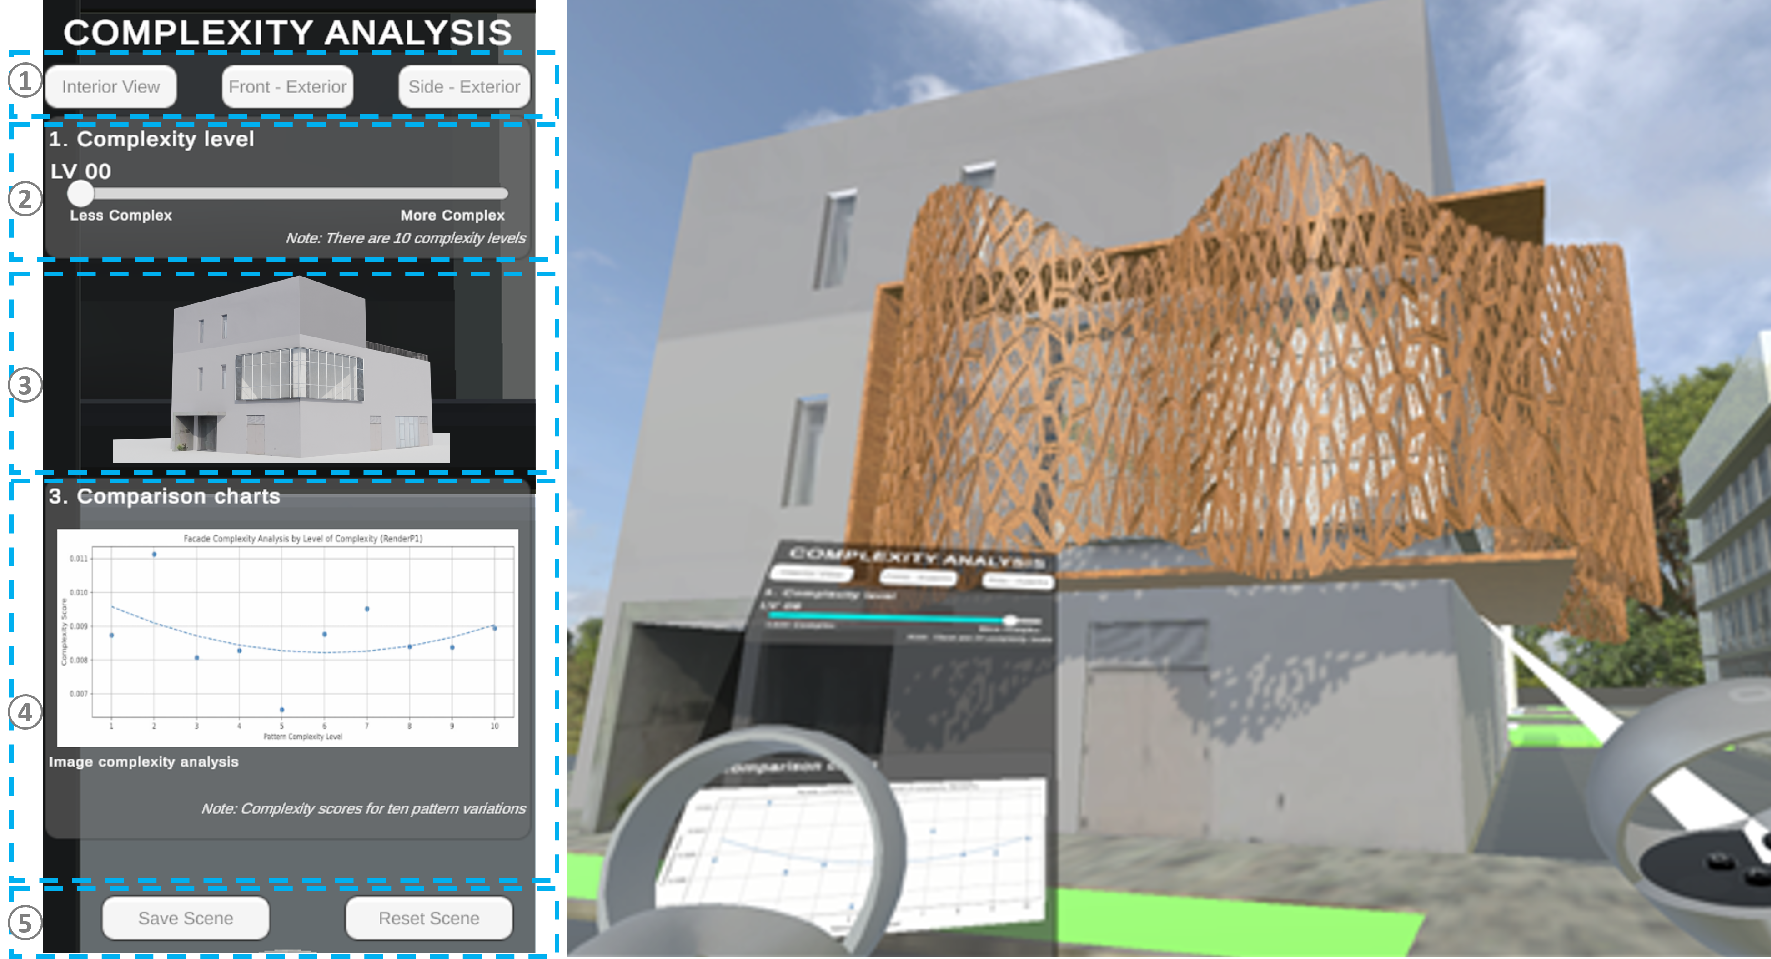
\includegraphics[width= \linewidth]{Images/VRInterface}
                \captionof{figure}{Detailed view of the VR interface (left) highlighting its five key sections: Viewpoint Navigation (1), Facade Variation Slider (2) for transitioning through ten facade variations, Facade Render Preview (3), Comparative Analysis Charts (4) displaying CICA complexity scores, and Utility Functions (5) for switching between the three patterns. Also shown are the VR simulations of the building's exterior (middle) and interior (right) as experienced during the facade complexity analysis, illustrating the transitions through various facade variations across all three patterns.}
                \label{fig:VRinterface}
            \end{minipage}
        \end{tabular}
    \end{table*}

    %!Figure of `Experiment Execution' flowchart
    %% Figure `Experiment Execution' flowchart
    %\begin{figure*}[htb]
%        \centering
%        \includegraphics[width= \linewidth]{Images/FlowchartExperiment}
%          \caption{`Experiment Execution' Flowchart: This flowchart outlines the three stages of the experiment, including the VR Interaction Stage (I), the Screen-Based Ranking Stage (II), and the Post-Experiment Survey (III), providing a visual representation of the sequential steps involved in the study.}
%          \label{fig:ExperimentFlowchart}
%    \end{figure*}


    \subsubsection{VR integration and simulation tools}
    \label{subsubsec:VR_integration}
    %%Define the sections of the VR interface and how information is displayed
    %\subsubsection{VR integration and data visualization interface}
%\label{subsubsec:VR_integration}
%%Define the sections of the VR interface and how information is displayed
%\input{Text/VR_integration}


The goal of this component is to integrate the virtual environment from the `3D Modeling and Environment Setup' with data from the CICA complexity analysis (Figure~\ref{fig:MethodologyFlowchart}, element 3).
This module features an immersive `VR simulation' and a `data visualization interface' that allows users to explore and interact with the building's interior and exterior, visualize its context, and manipulate facade variations (Figure~\ref{fig:VRinterface}).

The `VR simulation,' developed using Unity (v.2022.2.21f1) and accessible through a Head-Mounted Display (HMD) like the Oculus Quest 2, this software was chosen for its robust VR support, pre-built templates, and seamless integration with Python and C\#, enhancing simulation interactivity and data handling.

%!Vr interface
The VR data visualization interface provides real-time feedback on facade variations, facilitating data collection on user response to varying levels of facade complexity.
Structured into five key sections—Viewpoint Navigation, Facade Variation Slider, Facade Render Preview, CICA Scores Comparative Analysis Charts, and Utility Functions (labeled 1 to 5 in Figure~\ref{fig:VRinterface})—it enhances usability and interpretability, thereby optimizing the facade selection process.







    \subsection{Experiment Execution}
    \label{subsec:Experiment_execution}
    %%Task description, stage 1 to 3 with survey
    %\subsection{Experiment design}
%    \label{subsection:Experiment_design}
%    %%Task description, stage 1 to 3 with survey
%    %\subsection{Experiment design}
%    \label{subsection:Experiment_design}
%    %%Task description, stage 1 to 3 with survey
%    %\subsection{Experiment design}
%    \label{subsection:Experiment_design}
%    %%Task description, stage 1 to 3 with survey
%    \input{Text/ExperimentDesign}

With the VR system now comprehensively detailed, we transition into the experiment design phase, where we explore how this innovative virtual reality environment, equipped with the Computational Image Complexity Analysis (CICA) system-derived complexity data, will be utilized to investigate participants' responses to facade complexity variations.

This marks a pivotal stage in our study, where theory and technology converge to provide valuable insights into architectural complexity preferences.

The experiment is designed to comprehensively gauge participants' reactions to increasingly complex facade variations within immersive Virtual Reality simulations.
This process employs a Head-Mounted Display (HMD) and aims to quantitatively and qualitatively measure users' tolerance levels towards intricate facade designs (refer to Figure\ref{fig:ExperimentFlowchart}).

Conducted in our laboratory situated within the Architectural Environment Research Building, known as Building HE20, on the Itoshima campus of Kyushu University in Fukuoka, Japan, the experiment unfolds across three distinct stages: the `VR Interaction' stage, the `Screen-Based Ranking' stage, and the `Post-Experiment Survey' stage.

%% Figure Experiment Design flowchart
    \begin{figure}[htb]
      \centering
      % trim=left 190 down 250 right 150 top5
      \includegraphics[width= \linewidth, trim=0 0 0 0, clip]{Images/FlowchartExperiment}
      \caption{Flowchart illustrating the Experiment design stages, depicting the VR interaction stage, the Screen-based ranking stage and the Post-experiment survey.}
      \label{fig:ExperimentFlowchart}
    \end{figure}

%!VR interaction stage

In the initial stage of the experiment, participants were introduced to a Virtual Reality simulation that faithfully replicated the actual laboratory and building where they were invited to take part (Figure\ref{fig:VRInteriorExterior}).
Within this immersive environment, participants faced a distinctive challenge.
Their task was to select the most comfortable facade variation from a range of options presented in the virtual setting.

This scenario presented an intriguing question: if the laboratory were to become their permanent workplace or study location, how would participants choose a facade that would enhance their daily experience of entering the building and working within its confines, making it more comfortable and engaging?.

Participants were granted the freedom to incorporate their personal preferences into their final decisions, with a primary emphasis on enhancing workplace comfort.

To address this facade design selection challenge, participants were tasked with evaluating and selecting their preferred facade from three distinct patterns, each featuring ten variations labeled by complexity level (see \ref{sec:AnnexVariations}).
These patterns were presented in a randomized order to ensure unbiased results and were easily accessible as separate stages through the VR interface.

To provide participants with a heightened sense of realism and immersion, a section of the laboratory was cleared to allow them to physically move around within the virtual simulation of the lab.
This enabled them to gain a deeper understanding of how each facade variation would impact their environment.

This stage of the experiment yielded valuable insights into participants' complexity tolerance levels, extracted from their recorded selections of the facade variations they found most comfortable.


%! Screen-based ranking stage

After the conclusion of each of the three pattern stages in the VR system, participants proceeded to the `Screen-Based Ranking' stage of the experiment.

The primary objective of this stage was to assess the accuracy of the `Computational Image Complexity Analysis' (CICA) system in evaluating the complexity of facade variations in comparison to the perceptions of the participants.

In this stage, participants were presented with the same set of 10 facade variations that had been processed by the CICA system.
However, this time, the presentation format shifted to a screen-based interface, and participants used a mouse and keyboard to navigate through the images of the facade variations.

Their task was to independently analyze these variations and arrange them according to their personal judgments of complexity.
Participants were specifically instructed to disregard any aesthetic preferences when ranking the facades and concentrate solely on the degree of complexity, arranging them from the least complex (level 1) to the most complex (level 10).

This stage of the experiment was repeated three times, once for each of the three patterns.
The responses from participants were meticulously recorded and later used for evaluating the alignment between the participants' ranking assessments and those generated by the CICA system.

The primary goal of this analysis was to ascertain if there existed any notable disparities between the CICA system's rankings and the perceptions of the participants.
By scrutinizing the results of this ranking comparison, the study aimed to refine the Complexity Tolerance Metric derived from the first stage, adjusting it based on the margin of error resulting from the deviation observed in the second stage.
This refined metric provides a more precise basis for forecasting future trends in architectural construction, facilitating informed conclusions.

%! Post-experiment survey stage

The third and final stage of the experiment, known as the `Post-interaction Survey' stage, takes place after participants have completed both the Facade design selection task in the `VR interaction stage' and the facade variation ranking task in the `Screen-based ranking stage' for all three patterns.

This survey comprises 15 questions categorized into two sections: `Participant Background' and `Complexity Perception.'

The survey, provided in detail in \ref{sec:Annexsurvey}, serves a dual purpose.
Firstly, it aims to gather insights into the participants' professional backgrounds, including any prior experience they may have in addressing facade design-related challenges.
Secondly, it seeks to understand participants' perceptions of complexity in building design, shedding light on the decision-making processes that underlie their choices during the experiment.

The `Background section' encompasses 5 multiple-choice questions designed to identify participants' professional backgrounds and their previous involvement in solving facade design problems.

In contrast, the `Complexity perception section' features 10 questions measured on a 7-point Likert scale.
These questions delve into participants' qualitative perceptions of complexity when assessing a building.
Additionally, they help identify the key factors that influence their selection of a particular facade variation.

%! Metrics purpose

In summary, the comprehensive design of our experiment, consisting of three distinct stages - the `VR Interaction' stage, the `Screen-Based Ranking' stage, and the `Post-Experiment Survey' stage, is aimed at providing a multifaceted understanding of user tolerance for complex facades and its implications for future construction trends.

By integrating the quantitative data from the VR system, the ranking comparisons from the screen-based stage, and the qualitative responses from the survey, we can form a comprehensive understanding of user tolerance for complex facades.
We can also identify the drivers behind participants' preferences, shedding light on the evolving trends in future construction.

This combined analysis positions us to answer the core research question: What degree of complexity within facade design, would users tolerate and accept for a building, and what insights do their preferences provide for future architectural trends?' By combining quantitative and qualitative findings, we aim to provide a nuanced perspective that contributes to the discourse on architectural complexity and its implications for contemporary design and construction.





With the VR system now comprehensively detailed, we transition into the experiment design phase, where we explore how this innovative virtual reality environment, equipped with the Computational Image Complexity Analysis (CICA) system-derived complexity data, will be utilized to investigate participants' responses to facade complexity variations.

This marks a pivotal stage in our study, where theory and technology converge to provide valuable insights into architectural complexity preferences.

The experiment is designed to comprehensively gauge participants' reactions to increasingly complex facade variations within immersive Virtual Reality simulations.
This process employs a Head-Mounted Display (HMD) and aims to quantitatively and qualitatively measure users' tolerance levels towards intricate facade designs (refer to Figure\ref{fig:ExperimentFlowchart}).

Conducted in our laboratory situated within the Architectural Environment Research Building, known as Building HE20, on the Itoshima campus of Kyushu University in Fukuoka, Japan, the experiment unfolds across three distinct stages: the `VR Interaction' stage, the `Screen-Based Ranking' stage, and the `Post-Experiment Survey' stage.

%% Figure Experiment Design flowchart
    \begin{figure}[htb]
      \centering
      % trim=left 190 down 250 right 150 top5
      \includegraphics[width= \linewidth, trim=0 0 0 0, clip]{Images/FlowchartExperiment}
      \caption{Flowchart illustrating the Experiment design stages, depicting the VR interaction stage, the Screen-based ranking stage and the Post-experiment survey.}
      \label{fig:ExperimentFlowchart}
    \end{figure}

%!VR interaction stage

In the initial stage of the experiment, participants were introduced to a Virtual Reality simulation that faithfully replicated the actual laboratory and building where they were invited to take part (Figure\ref{fig:VRInteriorExterior}).
Within this immersive environment, participants faced a distinctive challenge.
Their task was to select the most comfortable facade variation from a range of options presented in the virtual setting.

This scenario presented an intriguing question: if the laboratory were to become their permanent workplace or study location, how would participants choose a facade that would enhance their daily experience of entering the building and working within its confines, making it more comfortable and engaging?.

Participants were granted the freedom to incorporate their personal preferences into their final decisions, with a primary emphasis on enhancing workplace comfort.

To address this facade design selection challenge, participants were tasked with evaluating and selecting their preferred facade from three distinct patterns, each featuring ten variations labeled by complexity level (see \ref{sec:AnnexVariations}).
These patterns were presented in a randomized order to ensure unbiased results and were easily accessible as separate stages through the VR interface.

To provide participants with a heightened sense of realism and immersion, a section of the laboratory was cleared to allow them to physically move around within the virtual simulation of the lab.
This enabled them to gain a deeper understanding of how each facade variation would impact their environment.

This stage of the experiment yielded valuable insights into participants' complexity tolerance levels, extracted from their recorded selections of the facade variations they found most comfortable.


%! Screen-based ranking stage

After the conclusion of each of the three pattern stages in the VR system, participants proceeded to the `Screen-Based Ranking' stage of the experiment.

The primary objective of this stage was to assess the accuracy of the `Computational Image Complexity Analysis' (CICA) system in evaluating the complexity of facade variations in comparison to the perceptions of the participants.

In this stage, participants were presented with the same set of 10 facade variations that had been processed by the CICA system.
However, this time, the presentation format shifted to a screen-based interface, and participants used a mouse and keyboard to navigate through the images of the facade variations.

Their task was to independently analyze these variations and arrange them according to their personal judgments of complexity.
Participants were specifically instructed to disregard any aesthetic preferences when ranking the facades and concentrate solely on the degree of complexity, arranging them from the least complex (level 1) to the most complex (level 10).

This stage of the experiment was repeated three times, once for each of the three patterns.
The responses from participants were meticulously recorded and later used for evaluating the alignment between the participants' ranking assessments and those generated by the CICA system.

The primary goal of this analysis was to ascertain if there existed any notable disparities between the CICA system's rankings and the perceptions of the participants.
By scrutinizing the results of this ranking comparison, the study aimed to refine the Complexity Tolerance Metric derived from the first stage, adjusting it based on the margin of error resulting from the deviation observed in the second stage.
This refined metric provides a more precise basis for forecasting future trends in architectural construction, facilitating informed conclusions.

%! Post-experiment survey stage

The third and final stage of the experiment, known as the `Post-interaction Survey' stage, takes place after participants have completed both the Facade design selection task in the `VR interaction stage' and the facade variation ranking task in the `Screen-based ranking stage' for all three patterns.

This survey comprises 15 questions categorized into two sections: `Participant Background' and `Complexity Perception.'

The survey, provided in detail in \ref{sec:Annexsurvey}, serves a dual purpose.
Firstly, it aims to gather insights into the participants' professional backgrounds, including any prior experience they may have in addressing facade design-related challenges.
Secondly, it seeks to understand participants' perceptions of complexity in building design, shedding light on the decision-making processes that underlie their choices during the experiment.

The `Background section' encompasses 5 multiple-choice questions designed to identify participants' professional backgrounds and their previous involvement in solving facade design problems.

In contrast, the `Complexity perception section' features 10 questions measured on a 7-point Likert scale.
These questions delve into participants' qualitative perceptions of complexity when assessing a building.
Additionally, they help identify the key factors that influence their selection of a particular facade variation.

%! Metrics purpose

In summary, the comprehensive design of our experiment, consisting of three distinct stages - the `VR Interaction' stage, the `Screen-Based Ranking' stage, and the `Post-Experiment Survey' stage, is aimed at providing a multifaceted understanding of user tolerance for complex facades and its implications for future construction trends.

By integrating the quantitative data from the VR system, the ranking comparisons from the screen-based stage, and the qualitative responses from the survey, we can form a comprehensive understanding of user tolerance for complex facades.
We can also identify the drivers behind participants' preferences, shedding light on the evolving trends in future construction.

This combined analysis positions us to answer the core research question: What degree of complexity within facade design, would users tolerate and accept for a building, and what insights do their preferences provide for future architectural trends?' By combining quantitative and qualitative findings, we aim to provide a nuanced perspective that contributes to the discourse on architectural complexity and its implications for contemporary design and construction.





%!text

The experiment is designed to assess participants' reactions to increasingly complex facade variations in VR simulations, using the CICA system-derived complexity data (element 3.2 in Figure~\ref{fig:MethodologyFlowchart}). It unfolds across three stages:

%!VR interaction stage
\begin{enumerate}
    \item \textit{`VR interaction' stage:}  as illustrated in the flowchart in Figure~\ref{fig:MethodologyFlowchart}~(element 3.2 I), participants were introduced to a VR simulation replicating the actual laboratory and building where the experiment took place (Figure~\ref{fig:VRinterface}).
    Their task was to select preferred facade variation from three patterns, each with ten complexity-labeled variations (Table~\ref{tab:PatternsVariationsPart0}) alongside data visualization of their CICA complexity score, considering the scenario where the laboratory would be their permanent workplace or study location.
    The patterns were presented in randomized order to ensure unbiased results and were accessible through the VR interface.
    The stage aims to gauge participants' complexity tolerance levels.
    \item \textit{`Screen-based Ranking' Stage:} As depicted in the flowchart in Figure~\ref{fig:MethodologyFlowchart}~(element 3.2 II), participants rank the same 10 facade variations based on their perception of complexity, through a screen-based interface, without CICA system data.
    This process was conducted for each of the three patterns.
    The aim of this analysis was to refine the CICA system's complexity analysis capabilities, thereby enhancing the accuracy of future architectural trend forecasts.
    \item \textit{`Post-interaction' Survey:} As shown in the flowchart in Figure~\ref{fig:MethodologyFlowchart}~(element 3.2 III), following the completion of the first two stages, participants answer a 15-question survey divided into Participant Background (Figures~\ref{fig:SurveyBackgroundChart}~\ref{fig:SurveyYearsExperienceChart}) and Complexity Perception sections (Figures~\ref{fig:SurveyQuestions6-10}~\ref{fig:SurveyQuestions11-15}) exploring participants' qualitative perceptions of complexity and the factors influencing their facade variation choices.
    This final section uses a 7-point Likert scale, chosen for its effectiveness in capturing detailed responses regarding complexity perception and element arrangement in facade design.
\end{enumerate}

%! Metrics purpose

The combined analysis of these stages aims to provide insights into user tolerance for complex facades and its implications for future construction trends.
By merging quantitative and qualitative findings, we contribute to the discourse on architectural complexity and its impact on contemporary design and construction.


    %!Table CICA scatter graph and table of Top and bottom scores for buildings
    % Table with figures and data from top 5 and bottom 5 CICA complexity scores of buildings from historical analysis
    \begin{table*}[!htb]
    \centering
    \small
    \begin{tabular}{c}
        %Top cell with one figure
        %Figure: CICA scatter graph for historical analysis
        \begin{minipage}{\textwidth}
            \centering
            \includegraphics[width= \linewidth]{Graphs/complexitygraph}
            \captionof{figure}{Scatter Graph of Architectural Complexity Over Time: This graph presents the CICA scores for 177 buildings, categorized by historical timeline and architectural style. An overlaid trendline highlights the current evolving trend towards increased complexity in architectural design as analyzed by the CICA system.}
            \label{fig:HistoricalComplexityGraph}
        \end{minipage}
        \\
        \\
        %2nd row with one table
        %Table: CICA top 5 buildings with year and scores
        \begin{minipage}{\textwidth}
            \centering
            \captionof{table}{Table of comparative CICA Historical Analysis results: Top 5 Highest and Bottom 5 Lowest CICA Complexity Scores from Historical Analysis, Including Year of Construction and Architectural Style.}
            \label{tab:Top5andBottom5CICAcomplexityScores}
            \begin{tabularx}{\linewidth}{c X c c c}
            \toprule
            \multicolumn{5}{c}{\textbf{Buildings with the Top 5 Highest CICA Complexity Scores}} \\
            \hline
            \textbf{Rank} & \textbf{Building Name} & \textbf{Year of Construction} & \textbf{Architectural Style} & \textbf{CICA Score} \\
            \hline
            1 & Westminster Abbey & 1245 & Gothic & 7.81 \\
            2 & Seattle Central Library & 2004 & Deconstructivism & 7.78 \\
            3 & Reims Kathedrale & 1275 & Gothic & 7.51 \\
            4 & California Academy of Sciences & 2008 & Hightech Modernism & 7.45 \\
            5 & Rome Trevi Fountain & 1732 & Baroque & 7.39 \\
            \hline
            \end{tabularx}
        \end{minipage}
        \\
        \\
        %3rd row cell with Figure
        %Figure CICA top 5 buildings
        \begin{minipage}{\textwidth}
            \centering
            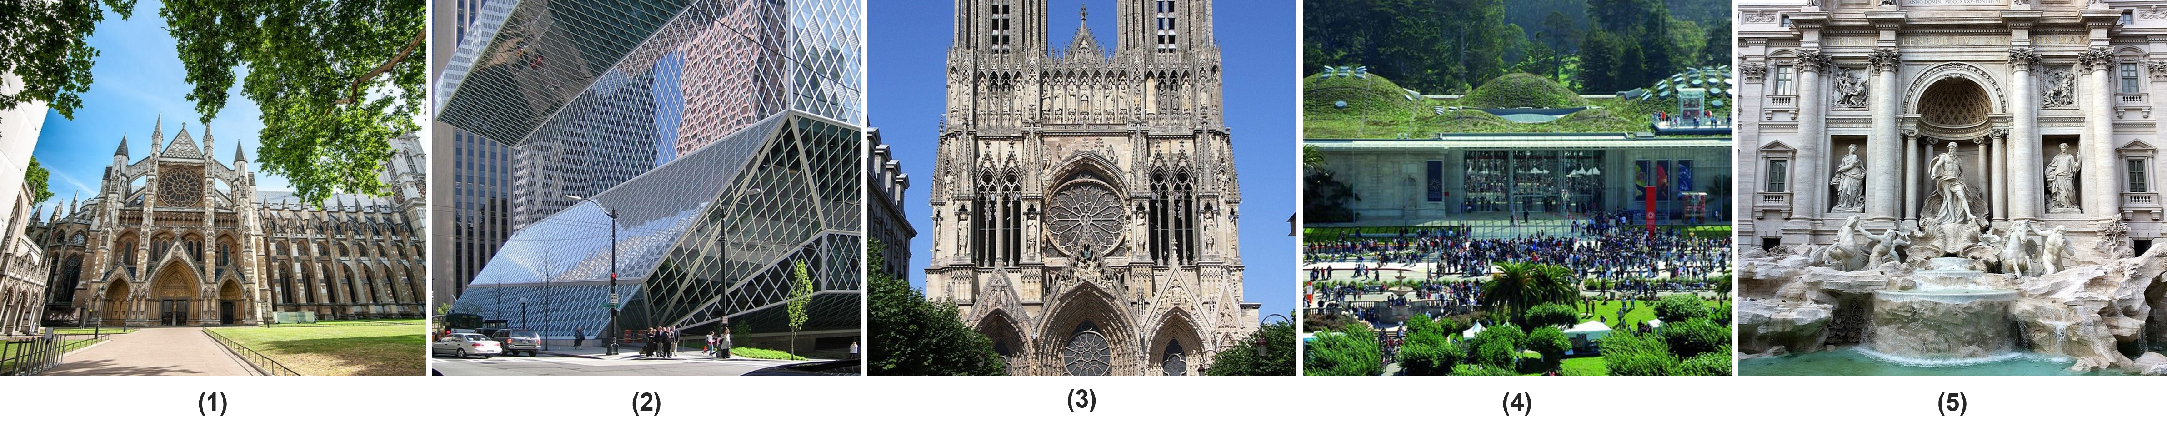
\includegraphics[width= \linewidth, trim=0cm 0.5cm 0cm 0.5cm]{Images/CICATop5}
            \label{fig:CICATop5scores}
        \end{minipage}
        \\
        %4rd row cell with Table
        %Table: CICA bottom 5 buildings with year and scores
        \begin{minipage}{\textwidth}
            \centering
            \begin{tabularx}{\linewidth}{c X c c c}
            \hline
            \multicolumn{5}{c}{\textbf{Buildings with the Bottom 5 Lowest CICA Complexity Scores}} \\
            \hline
            \textbf{Rank} & \textbf{Building Name} & \textbf{Year of Construction} & \textbf{Architectural Style} & \textbf{CICA Score} \\
            \hline
            1 & Luce Memorial Chapel, Taichung City, Taiwan & 1963 & Modernism & 0.66 \\
            2 & Imperial War Museum North & 2002 & Deconstructivism & 0.79 \\
            3 & St. Mary's Cathedral, Tokyo & 1964 & Modernism & 1.07 \\
            4 & Disney Concert Hall & 2003 & Deconstructivism & 1.13 \\
            5 & Cathedral of Brasilia in Brazil & 1970 & Modernism & 1.22 \\
            \bottomrule
            \end{tabularx}
        \end{minipage}
        \\
        \\
        %Bottom cell with Figure
        %Figure CICA top 5 buildings
        \begin{minipage}{\textwidth}
            \centering
            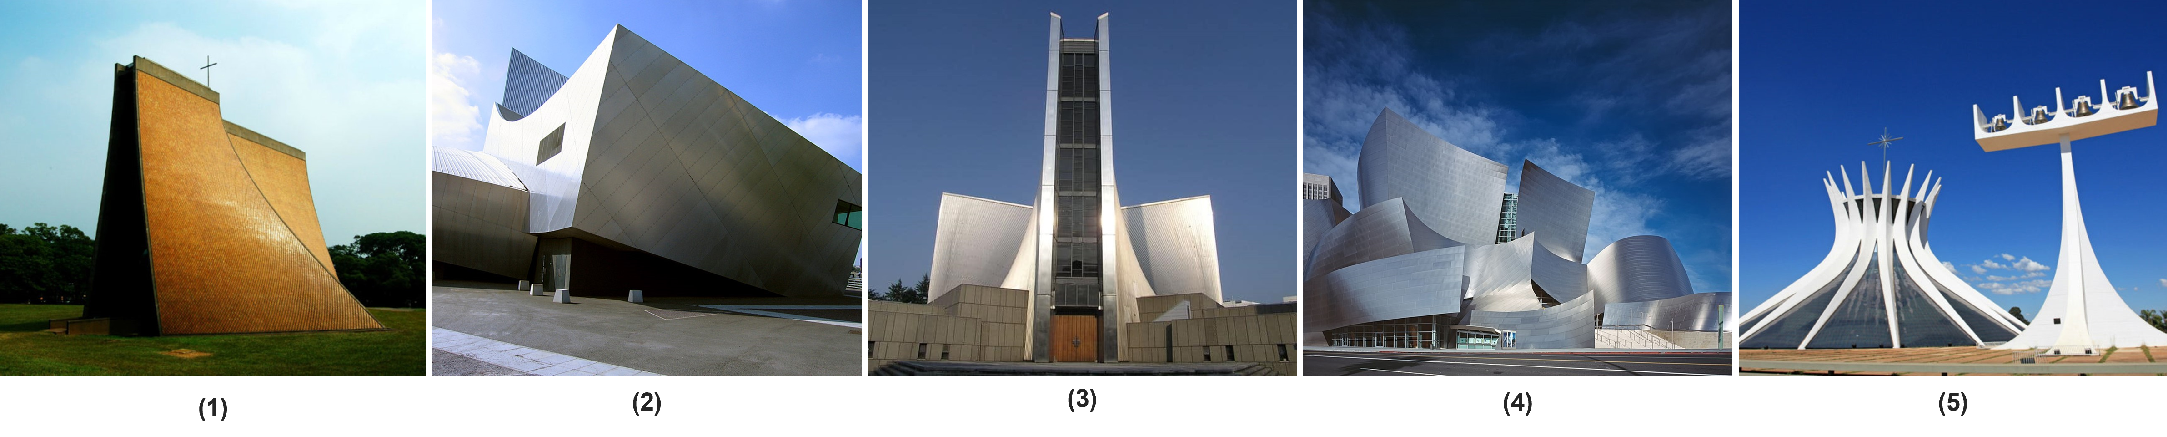
\includegraphics[width= \linewidth, trim=0cm 0.5cm 0cm 0.5cm]{Images/CICABottom5}
            \label{fig:CICABottom5scores}
        \end{minipage}
    \end{tabular}
    \end{table*}

    \subsection{Data Analysis and Validation}
    \label{subsec:Data_analysis}
    The final phase of our methodology involves a detailed analysis of the data collected during the experiments, crucial for validating the effectiveness of the `Complexity Analysis' system in evaluating facades.

It is structured as follows:

\begin{enumerate}
    \item \textit{Data Processing and Analysis:} ...Advanced statistical tools
    \item \textit{Performance Evaluation:} We assess the `Complexity Analysis' system's impact on user by examining:
        \begin{itemize}
            \item \textit{Accuracy Analysis:} ...
            \item \textit{Participant Perception Survey:} ...
        \end{itemize}

        These metrics are critical

    \item \textit{Results Interpretation and Reporting:} Data synthesis ...
\end{enumerate}

%Closing statement

%

\section{Results and Discussion}
\label{sec:Results}
%% Results should be clear and concise.
%!\section{Results}
%\label{sec:Results}
%%!\section{Results}
%\label{sec:Results}
%%!\section{Results}
%\label{sec:Results}
%\input{text/RD_1Results_DiscussionIntro.tex}

%=============================
%%% Results should be clear and concise.
%Report the results of the study
%Report main findings concisely in a logical order

% Intro ===============

Building upon the methodologies outlined in the previous sections, this section presents findings from two primary sources: the application of the CICA system to a historical dataset of architectural images across various epochs and styles, and data collected from the experiment designed to gauge user responses to facade complexity.
Organized according to the goals set forth in the introduction, this section elucidates the evolving relationship between users and architectural complexity, providing valuable insights for future construction practices and the quantification of complexity in facade design.

%!Goals oriented discussion






%=============================
%%% Results should be clear and concise.
%Report the results of the study
%Report main findings concisely in a logical order

% Intro ===============

Building upon the methodologies outlined in the previous sections, this section presents findings from two primary sources: the application of the CICA system to a historical dataset of architectural images across various epochs and styles, and data collected from the experiment designed to gauge user responses to facade complexity.
Organized according to the goals set forth in the introduction, this section elucidates the evolving relationship between users and architectural complexity, providing valuable insights for future construction practices and the quantification of complexity in facade design.

%!Goals oriented discussion






%=============================
%%% Results should be clear and concise.
%Report the results of the study
%Report main findings concisely in a logical order

% Intro ===============

Building upon the methodologies outlined in the previous sections, this section presents findings from two primary sources: the application of the CICA system to a historical dataset of architectural images across various epochs and styles, and data collected from the experiment designed to gauge user responses to facade complexity.
Organized according to the goals set forth in the introduction, this section elucidates the evolving relationship between users and architectural complexity, providing valuable insights for future construction practices and the quantification of complexity in facade design.

%!Goals oriented discussion






    \subsection{Assessment and Implications of Facade Complexity across Architectural Eras using the CICA System and insights from literature review}
    \label{subsec:ResultsComplexityImageAnalysishistory}
    %!\subsection{Assessment and Implications of Facade Complexity across Architectural Eras using the CICA System and insights from literature review}
%    \label{subsec:ResultsComplexityImageAnalysishistory}
%    %!\subsection{Quantitative complexity Analysis}
%    \label{subsec:ComplexityImageAnalysis}
%    %!\subsection{Quantitative complexity Analysis}
%    \label{subsec:ComplexityImageAnalysis}
%    \input{Text/RD_ResultsCICAHistory.tex}
%% Figure of Complexity graph

We have previously discussed that architectural evolution has been characterized by a continual interplay between simplicity and complexity.
Our literature review, presented in Section \ref{sec:Literature review}, has consistently pointed towards a prevailing trend in contemporary architecture, suggesting a resurgence of complexity in architectural design.

Our initial hypothesis, grounded in a rigorous examination of architectural styles from a theoretical standpoint, detailed in Section \ref{subsec:TimelineArchitectureStyles}, suggests that architecture undergoes cyclical oscillations between simplicity and complexity.
In the post-modern era, we posited that contemporary architecture would witness a resurgence of complexity and ornamentation.
This resurgence is exemplified by the emergence of five prominent styles: Deconstructivism, Neofuturism, High-tech Modernism, Parametricism, and Pragmatic Utopianism (see Figure \ref{fig:contemporarytimeline}).

These styles are influenced by technological advancements, the widespread use of computer-aided design tools, and a growing focus on sustainability.
Together, these factors contribute to a contemporary architectural landscape characterized by increasing complexity.

\textbf{CICA System for Quantitative Assessment}

While defining architectural complexity is inherently challenging due to its interconnection with various socio-economic factors influencing urban development, the development of the CICA system was based on a premise.
By accumulating a vast and diverse dataset of architectural works from different centuries, we aimed to uncover discernible patterns that would validate our hypothesis: architecture is characterized by a continuous dialogue between simplicity and complexity, with a trend towards increased complexity in contemporary architecture.

To objectively validate this trend, we conducted a quantitative analysis using the CICA system.
This rigorous analysis method utilizes input images of the most iconic and representative buildings from various epochs and styles, totaling 177 buildings across 14 architectural styles(illustrated in timelines in Figure \ref{fig:Oldtimeline}, \ref{fig:Middletimeline}, \ref{fig:contemporarytimeline}).
The CICA system took only 4.54 seconds to calculate the CICA scores for all the buildings and plot the graph, demonstrating its efficiency for complexity analysis.

The results are visually depicted in the scatter graph titled `Architectural Complexity over time' in Figure \ref{fig:HistoricalComplexityGraph}, and a 9th-degree polynomial trendline was found to be the best fit due to its versatility in accommodating the intricate data patterns that naturally emerge when assessing historical building complexity scores, the outcome of this choice was the emergence of a curve characterized by an intriguing cyclic pattern.

The distinctive pattern found on the trendline, akin to an undulating curve, uncovers a continual oscillation between architectural complexity and simplicity.
It resembles the paradigmatic shifts in architectural design discussed within our theoretical analysis (see section\ref{subsec:FacadeandOrnament}), a phenomenon that has endured throughout architectural history.

\textbf{Periods of Rapid Change:}
The polynomial curve in the 'Historical Complexity Analysis' Chart (Figure \ref{fig:HistoricalComplexityGraph}) reveals a dynamic oscillation between periods of ornamental richness and minimalist restraint, illustrating the unique interpretation of architectural complexity in each historical era.

Notably, the late 20th century show spikes in complexity scores, indicating significant shifts in architectural trends associated with the transition from the minimalist aesthetics of Modernism to the more eclectic and elaborate designs of Postmodernism.
Additionally, a shift is observed from the Gothic to the Renaissance period, where the trendline peaks with the ornate and vertical architecture of the Gothic era and descends as the Renaissance favors harmony, proportion, and classical simplicity \cite{Stacbond2020}.

Furthermore, our analysis of the last 50 years of data reveal an upward trajectory in architectural complexity, marking a departure from the minimalism of the 1950s and 1960s Modernist movement.
This trend supports our hypothesis and underscores the cyclical nature of architectural complexity, reflecting ongoing dialogues within architectural practice throughout history.

\textbf{Outliers:} Certain buildings stand out with exceptionally high or low complexity scores, warranting individual examination to understand their unique design elements or historical context.
Our investigation into the extremes of architectural complexity, as evidenced by the top 5 highest and bottom 5 lowest CICA scores (refer to Table \ref{tab:Top5andBottom5CICAcomplexityScores}), reveals significant outliers that deviate from the predominant complexity trends identified in our historical analysis.

Westminster Abbey, constructed in 1245 and exemplifying the Gothic architectural style, tops the chart with the highest CICA complexity score of 7.81 (Table \ref{tab:Top5andBottom5CICAcomplexityScores}, Top (1)).
This result underscores the intricate design characteristic of the Gothic period, known for its detailed stonework and skyward designs\cite{Stacbond2020}.

Conversely, the Luce Memorial Chapel in Taichung City, Taiwan, represents the other extreme, obtaining the lowest CICA complexity score of 0.66.
Built in 1963, this Modernist building exemplifies the minimalist ethos of the time, focusing on simplicity and functionality(Table \ref{tab:Top5andBottom5CICAcomplexityScores}, Bottom (1)).

These two buildings, marking the highest and lowest complexity scores in our study, illustrate the broad spectrum of architectural styles and the associated complexity over time and serve as critical case studies for understanding the factors that drive exceptional complexity or simplicity in architectural design.

%%Continue here

%\textbf{Correlation with Historical Events:} The complexity trends appear to correlate with major historical events, such as the industrial revolution and the advent of digital design technologies, influencing architectural design approaches.

%!Gothic Period
%Medieval Period (12th to 16th Century): Gothic architecture emerged in the High and Late Middle Ages, a time characterized by a growth in population, trade, and the establishment of universities. The period saw a shift from the Romanesque style to the Gothic style, which was marked by innovations such as the pointed arch, ribbed vault, and flying buttress. These architectural advancements allowed for taller, more light-filled structures, which were often used in the construction of cathedrals and churches.
%
%Crusades (11th to 13th Century): The Crusades played a role in the cultural exchange between the East and West. The exposure to Eastern architectural styles and techniques may have influenced the development of Gothic architecture in Europe. The increased wealth from trade and the need for monumental religious structures to demonstrate piety and power also contributed to the flourishing of Gothic architecture.


%!Renaissance
%Enlightenment (Illuminism) (Late 17th to 18th Century): This period emphasized reason, science, and individualism, which could have influenced a shift towards more rational and less ornate architectural designs.

%!Neo-classical and eclectic naturalism
%Industrial Revolution (Late 18th to Early 19th Century): The advent of new building materials like iron and steel, along with advancements in construction techniques, enabled more complex and innovative architectural designs.

%!International style and modernism
%World War I (1914-1918) and World War II (1939-1945): The wars and their aftermaths led to a focus on functionality and austerity in architecture, contributing to the rise of Modernism and its emphasis on simplicity.

%!Post modernism and contemporar styles
%Advent of Computers (Mid-20th Century Onwards): The introduction of computer-aided design (CAD) tools allowed architects to explore more complex and intricate designs, contributing to the rise of styles like Deconstructivism and Parametricism.
%
%Post-Industrialization and Globalization (Late 20th to Early 21st Century): These phenomena have led to a more interconnected world, with a diverse range of architectural styles and a trend towards complexity in design to accommodate new urban and environmental challenges.










%% Figure of Complexity graph

We have previously discussed that architectural evolution has been characterized by a continual interplay between simplicity and complexity.
Our literature review, presented in Section \ref{sec:Literature review}, has consistently pointed towards a prevailing trend in contemporary architecture, suggesting a resurgence of complexity in architectural design.

Our initial hypothesis, grounded in a rigorous examination of architectural styles from a theoretical standpoint, detailed in Section \ref{subsec:TimelineArchitectureStyles}, suggests that architecture undergoes cyclical oscillations between simplicity and complexity.
In the post-modern era, we posited that contemporary architecture would witness a resurgence of complexity and ornamentation.
This resurgence is exemplified by the emergence of five prominent styles: Deconstructivism, Neofuturism, High-tech Modernism, Parametricism, and Pragmatic Utopianism (see Figure \ref{fig:contemporarytimeline}).

These styles are influenced by technological advancements, the widespread use of computer-aided design tools, and a growing focus on sustainability.
Together, these factors contribute to a contemporary architectural landscape characterized by increasing complexity.

\textbf{CICA System for Quantitative Assessment}

While defining architectural complexity is inherently challenging due to its interconnection with various socio-economic factors influencing urban development, the development of the CICA system was based on a premise.
By accumulating a vast and diverse dataset of architectural works from different centuries, we aimed to uncover discernible patterns that would validate our hypothesis: architecture is characterized by a continuous dialogue between simplicity and complexity, with a trend towards increased complexity in contemporary architecture.

To objectively validate this trend, we conducted a quantitative analysis using the CICA system.
This rigorous analysis method utilizes input images of the most iconic and representative buildings from various epochs and styles, totaling 177 buildings across 14 architectural styles(illustrated in timelines in Figure \ref{fig:Oldtimeline}, \ref{fig:Middletimeline}, \ref{fig:contemporarytimeline}).
The CICA system took only 4.54 seconds to calculate the CICA scores for all the buildings and plot the graph, demonstrating its efficiency for complexity analysis.

The results are visually depicted in the scatter graph titled `Architectural Complexity over time' in Figure \ref{fig:HistoricalComplexityGraph}, and a 9th-degree polynomial trendline was found to be the best fit due to its versatility in accommodating the intricate data patterns that naturally emerge when assessing historical building complexity scores, the outcome of this choice was the emergence of a curve characterized by an intriguing cyclic pattern.

The distinctive pattern found on the trendline, akin to an undulating curve, uncovers a continual oscillation between architectural complexity and simplicity.
It resembles the paradigmatic shifts in architectural design discussed within our theoretical analysis (see section\ref{subsec:FacadeandOrnament}), a phenomenon that has endured throughout architectural history.

\textbf{Periods of Rapid Change:}
The polynomial curve in the 'Historical Complexity Analysis' Chart (Figure \ref{fig:HistoricalComplexityGraph}) reveals a dynamic oscillation between periods of ornamental richness and minimalist restraint, illustrating the unique interpretation of architectural complexity in each historical era.

Notably, the late 20th century show spikes in complexity scores, indicating significant shifts in architectural trends associated with the transition from the minimalist aesthetics of Modernism to the more eclectic and elaborate designs of Postmodernism.
Additionally, a shift is observed from the Gothic to the Renaissance period, where the trendline peaks with the ornate and vertical architecture of the Gothic era and descends as the Renaissance favors harmony, proportion, and classical simplicity \cite{Stacbond2020}.

Furthermore, our analysis of the last 50 years of data reveal an upward trajectory in architectural complexity, marking a departure from the minimalism of the 1950s and 1960s Modernist movement.
This trend supports our hypothesis and underscores the cyclical nature of architectural complexity, reflecting ongoing dialogues within architectural practice throughout history.

\textbf{Outliers:} Certain buildings stand out with exceptionally high or low complexity scores, warranting individual examination to understand their unique design elements or historical context.
Our investigation into the extremes of architectural complexity, as evidenced by the top 5 highest and bottom 5 lowest CICA scores (refer to Table \ref{tab:Top5andBottom5CICAcomplexityScores}), reveals significant outliers that deviate from the predominant complexity trends identified in our historical analysis.

Westminster Abbey, constructed in 1245 and exemplifying the Gothic architectural style, tops the chart with the highest CICA complexity score of 7.81 (Table \ref{tab:Top5andBottom5CICAcomplexityScores}, Top (1)).
This result underscores the intricate design characteristic of the Gothic period, known for its detailed stonework and skyward designs\cite{Stacbond2020}.

Conversely, the Luce Memorial Chapel in Taichung City, Taiwan, represents the other extreme, obtaining the lowest CICA complexity score of 0.66.
Built in 1963, this Modernist building exemplifies the minimalist ethos of the time, focusing on simplicity and functionality(Table \ref{tab:Top5andBottom5CICAcomplexityScores}, Bottom (1)).

These two buildings, marking the highest and lowest complexity scores in our study, illustrate the broad spectrum of architectural styles and the associated complexity over time and serve as critical case studies for understanding the factors that drive exceptional complexity or simplicity in architectural design.

%%Continue here

%\textbf{Correlation with Historical Events:} The complexity trends appear to correlate with major historical events, such as the industrial revolution and the advent of digital design technologies, influencing architectural design approaches.

%!Gothic Period
%Medieval Period (12th to 16th Century): Gothic architecture emerged in the High and Late Middle Ages, a time characterized by a growth in population, trade, and the establishment of universities. The period saw a shift from the Romanesque style to the Gothic style, which was marked by innovations such as the pointed arch, ribbed vault, and flying buttress. These architectural advancements allowed for taller, more light-filled structures, which were often used in the construction of cathedrals and churches.
%
%Crusades (11th to 13th Century): The Crusades played a role in the cultural exchange between the East and West. The exposure to Eastern architectural styles and techniques may have influenced the development of Gothic architecture in Europe. The increased wealth from trade and the need for monumental religious structures to demonstrate piety and power also contributed to the flourishing of Gothic architecture.


%!Renaissance
%Enlightenment (Illuminism) (Late 17th to 18th Century): This period emphasized reason, science, and individualism, which could have influenced a shift towards more rational and less ornate architectural designs.

%!Neo-classical and eclectic naturalism
%Industrial Revolution (Late 18th to Early 19th Century): The advent of new building materials like iron and steel, along with advancements in construction techniques, enabled more complex and innovative architectural designs.

%!International style and modernism
%World War I (1914-1918) and World War II (1939-1945): The wars and their aftermaths led to a focus on functionality and austerity in architecture, contributing to the rise of Modernism and its emphasis on simplicity.

%!Post modernism and contemporar styles
%Advent of Computers (Mid-20th Century Onwards): The introduction of computer-aided design (CAD) tools allowed architects to explore more complex and intricate designs, contributing to the rise of styles like Deconstructivism and Parametricism.
%
%Post-Industrialization and Globalization (Late 20th to Early 21st Century): These phenomena have led to a more interconnected world, with a diverse range of architectural styles and a trend towards complexity in design to accommodate new urban and environmental challenges.










%% Figure of Complexity graph


While defining architectural complexity is inherently challenging due to its interconnection with various socio-economic and cultural factors influencing urban development, the CICA system was developed on the premise that analyzing a vast and diverse dataset of architectural works from different centuries could reveal patterns validating our hypothesis.
This hypothesis, established on the literature review (Section~\ref{subsec:TimelineArchitectureStyles}), suggests a cyclical nature in architecture—an ongoing dialogue between simplicity and complexity—with a trend towards increased complexity in contemporary architecture.
This trend is evidenced by recent architectural styles (see Figure~\ref{fig:contemporarytimeline}), influenced by technological advancements, computer-aided design tools, and a growing focus on sustainability.

\textbf{CICA System for Quantitative Assessment}

To validate this trend objectively, we conducted a quantitative analysis using the CICA system.
This analysis utilized images of 177 iconic buildings across 14 architectural styles (samples illustrated in Figures~\ref{fig:Earlytimeline},~\ref{fig:Transitionaltimeline},~\ref{fig:contemporarytimeline}). The CICA system calculated the complexity scores for all buildings and plotted the graph in just 4.54 seconds, demonstrating its efficiency.

The results are depicted in the scatter graph `Historical Analysis of Architectural Complexity Trends Over Time' in Figure~\ref{fig:HistoricalComplexityGraph}.
A 9th-degree polynomial trendline, best accommodating the intricate data patterns, revealed a distinctive undulating curve.
This pattern validates our hypothesis of continual oscillation between architectural complexity and simplicity, aligning with the paradigmatic shifts discussed in the Literature Review (Section~\ref{subsec:TimelineArchitectureStyles}) and showcasing a trend towards complexity in the post-modern era.

\textbf{Periods of Rapid Change:}

The trendline in the `Historical Analysis of Architectural Complexity Trends Over Time' Chart (Figure~\ref{fig:HistoricalComplexityGraph}) reveals dynamic oscillations between periods of ornamental richness and minimalist restraint, illustrating the unique interpretation of architectural complexity in each era.
Notably, a shift is observed from the Gothic to the Renaissance period, where the trendline peaks with the ornate and vertical architecture of the Gothic era~\cite{Kennedy2013} and descends as the Renaissance favors harmony, proportion, and classical simplicity~\cite{Marder1990}.
Additionaly, the late 20th century shows spikes in complexity scores, indicating significant shifts in architectural trends associated with the transition from the minimalist aesthetics of Modernism to the more eclectic and elaborate designs of Postmodernism.
Furthermore, our analysis of the last 50 years of data reveal an upward trajectory in architectural complexity, marking a departure from the uniformity of barren walls and fully glazed facades.

\textbf{Outliers:}

Certain buildings stand out with exceptionally high or low CICA scores, warranting individual examination.
Our investigation into these extremes, as evidenced by the top 5 highest and bottom 5 lowest CICA scores (Table~\ref{tab:Top5andBottom5CICAcomplexityScores}), reveals significant outliers.
Westminster Abbey, exemplifying Gothic architecture, tops the chart with the highest complexity score of 7.81, underscoring the intricate design characteristic of the Gothic period~\cite{Kennedy2013}.
Conversely, the Luce Memorial Chapel in Taichung City, Taiwan, built in 1963, represents the minimalist ethos of the time with the lowest complexity score of 0.66.
These buildings illustrate the broad spectrum of architectural styles and associated complexity over time, serving as critical case studies for understanding exceptional complexity or simplicity in design.






    %!Figures of experiment results 1
    %Table 2x3 Results part 1
    %Participant background chart, years of experience, Bar Chart of Chosen facade variation, Probability Chart and Complexity level per Pattern
    \begin{table*}[!htb]
        \centering
        \small
        \begin{tabular}{c}
            %Top cell with two nested figures side by side
            %Participants background and Years of experience
            \begin{minipage}{\textwidth}
                \centering
                % Left figure
                %Participants background
                \begin{minipage}{0.49\textwidth}
                    \includegraphics[width=\linewidth, trim=0 0 0 0]{Images/SurveyBackground}
                    \captionof{figure}{Participants' Background:This pie chart shows the distribution of participants' backgrounds, with architects(34\%) and undergraduate students(22\%) as the predominant groups (26 participants).}
                    \label{fig:SurveyBackgroundChart}
                \end{minipage}
                \hfill % Spacing between the figures
                % Right figure
                % Years of experience
                \begin{minipage}{0.49\textwidth}
                    \includegraphics[width=\linewidth, trim=0 0 0 0]{Images/SurveyExperience}
                    \captionof{figure}{Participants' Professional Experience in Facade Design: This pie chart displays the distribution of experience levels, with 86\% having none and 14\% having 1--5 years of experience (26 participants).}
                    \label{fig:SurveyYearsExperienceChart}
                \end{minipage}
            \end{minipage}
            \\
            %Middle cell with one figure
            %Facade chosen and CICA score chart per participant
            \begin{minipage}{\textwidth}
                \centering
                \includegraphics[width=\linewidth]{Images/ComplexityLevelChosenChart}
                \captionof{figure}{Facade Variation Selections and CICA Scores During VR Stage: This chart shows participants' chosen facade variations (bars, height = ID number 1--10) and their CICA complexity scores (line, points = score 0--10) during the VR stage of the experiment. The solid line represents individual CICA scores, while the dotted line indicates the mean average. This visualization highlights the relationship between participant selections and complexity assessment in the immersive VR environmentChart displaying participants' preferred complexity levels among the ten options during the VR simulation stage of the experiment for all three patterns.(CICA Score: Mean = 4.05; SD = 1.2) (26 participants, 78 experiment sessions)}
                \label{fig:ComplexityLevelChosenChart}
            \end{minipage}
            \\
            %Bottom cell with two nested figures side by side
            %Probability Chart and Complexity level per Pattern
            \begin{minipage}{\textwidth}
                \centering
                % Left figure
                % Probability Chart
                \begin{minipage}{0.49\textwidth}
                    \includegraphics[width=\linewidth]{Images/ProbabilityPreferredComplexitylevel}
                    \captionof{figure}{This scatter graph illustrates the probability distribution of preferred CICA scores for facade design across all three patterns, based on data collected during the VR stage of the experiment. (CICA score: \(Mean = 4.05, with Probabilty = 40\%\ ; SD = 12\%\)) (26 participants)}
                    \label{fig:ProbabilityComplexitylevelChart}
                \end{minipage}
                \hfill % Spacing between the figures
                % Right figure
                % Complexity level per Pattern
                \begin{minipage}{0.49\textwidth}
                    \includegraphics[width=\linewidth]{Images/PreferredComplexityLevelPerPattern}
                    \captionof{figure}{This bar chart presents the average chosen facade variation and corresponding CICA scores per pattern, as selected by participants during the VR stage of the experiment. (Facade variation: \(Mean = 4.4\)) (dotted line, CICA score: \(Mean = 4.05; SD = 1.2\)) (26 participants).}
                    \label{fig:ComplexityLevelPerPattern}
                \end{minipage}
            \end{minipage}
        \end{tabular}
    \end{table*}

    %!Figures of experiment results 2
    %Table 1x2
    % Accuracy graphs of complexity ranking per pattern
    \begin{table*}[!htb]
        \centering
        \small
        \begin{tabular}{c}
            %Top cell with one figure
            %Accuracy graphs of complexity ranking per pattern as a single image
            \begin{minipage}{\textwidth}
                \centering
                \includegraphics[width=\linewidth]{Images/AccuracyPatternMaster}
                \captionof{figure}{Comparative Analysis of Perceived Complexity vs. CICA Complexity Scores per Pattern: This line graph series illustrates the difference between participants' perceived complexity rankings and the objective CICA scores for facade variations within three distinct patterns. The graphs are presented from left to right: Pattern 1 (a), Pattern 2 (b), and Pattern 3 (c). The ranking line shows the complexity assessment from least (1) to most complex (10),highlighting the contrast between human perception and computational analysis in evaluating architectural complexity (26 participants).}
                \label{fig:AccuracyPatternMaster}
            \end{minipage}
        \end{tabular}
    \end{table*}

%!Figures of survey results
    % Survey question graph
    \begin{table*}[!htb]
        \centering
        \small
        \begin{tabular}{c}
            %Top cell with figures side by side
            %Survey question graphs
            \begin{minipage}{\textwidth}
                \centering
                % Left figure
                % Survey question 6 to 10
                \begin{minipage}{0.49\textwidth}
                    \includegraphics[width=\linewidth]{Images/SurveyPart1Complexity}
                    \captionof{figure}{Questions 6 to 10 of the Complexity perception section from the Post-Experiment Survey. \- (n = 10), 1 - strongly disagree, 7 - strongly agree.}
                    \label{fig:SurveyQuestions6-10}
                \end{minipage}
                \hfill % Spacing between the figures
                % Right figure
                % Survey question 11 to 15
                \begin{minipage}{0.49\textwidth}
                    \includegraphics[width=\linewidth]{Images/SurveyPart2Complexity}
                    \captionof{figure}{Questions 11 to 15 of the Complexity perception section from the Post-Experiment Survey. \- (n = 10), 1 - strongly disagree, 7 - strongly agree.}
                    \label{fig:SurveyQuestions11-15}
                \end{minipage}
            \end{minipage}
        \end{tabular}
    \end{table*}

    \subsection{Quantitative Analysis on Users Response to Complex Facades}
    \label{subsec:ResultsExperiment}
    %\section{Results}
%\label{sec:Results}
%% Results should be clear and concise.

%! Text
The experiment was carried out at Kyushu University, Fukuoka, Japan.
The study took place in two timeframes, from October 12 to October 30, 2023, and July 1 to July 12, 2024, with experiments held between 10:00 and 18:00.

A total of 26 participants, comprising university students and faculty members, engaged in the experiment.
The demographic distribution of the participants is illustrated in Figure~\ref{fig:SurveyBackgroundChart}.
The majority (67\%) were students from various disciplines, while 33\% had a background in construction, and 14\% had prior experience in facade design, as depicted in Figure~\ref{fig:SurveyYearsExperienceChart}.

\textbf{VR to measure user tolerance and preference for complexity in facade design.}

In the VR Interaction stage, participants engaged with the facade selection task for all three patterns, resulting in 78 experiment sessions.
For each pattern, participants selected the facade variation they found most comfortable based on its perceived complexity level.

%!Complexity level chosen bar chart

The preferred complexity levels from the VR simulation stage were consolidated into the `Facade variatio selection and CICA score Chart,' a bar chart, shown in Figure~\ref{fig:ComplexityLevelChosenChart}.
Analysis of this chart reveals that most participants favored one of the first five facade variations, with only five instances selecting options beyond this range.
On average, participants preferred a complexity score level of \(Mean = 3.82\) with a standard deviation of \(SD = 1.1\), as determined by the CICA system.
Notably, `facade variation 3'  emerged as the most popular choice for all three patterns among the ten defined complexity levels (see Table~\ref{tab:PatternsVariationsPart1} in~\ref{sec:AnnexVariations}).

%!Complexity level chosen probability graph

The `Probability Distribution Graph of Preferred CICA Scores Across Patterns', showcased in Figure~\ref{fig:ProbabilityComplexitylevelChart}, provides a visual representation of the distribution of participant choices.
It accentuates that there is a \(40\%\) probability of the focus group selecting an answer proximate to the calculated complexity score average,\(Mean = 3.82\) with a modest standard deviation of \(SD = 13\%\) in predicting individual data points or outcomes.
 This indicates a moderate level of predictability in participant choices based on the CICA system's complexity assessment.

%!Comparison chart of Average Chosen Facade and CICA scores by pattern

The `Comparison chart of Average Chosen Facade and CICA scores by pattern', displayed in Figure~\ref{fig:ComplexityLevelPerPattern}, underscores that the average choice of facade variation for each pattern hovers around the overall average complexity score, \(Mean = 3.82\) and the average choice of facade variation \(Mean = 3.9\), further supporting the alignment between participant preferences and the CICA system's complexity evaluation.

%Preliminary conclsuions from quantitative results

The results from these preliminary analysis indicate a preference among participants for facades with moderate complexity, hinting at a future architectural trend that favors a harmonious balance between intricacy and simplicity.
Such designs are likely to be visually engaging without being overwhelming.
Additionally, the diversity in participant responses suggests a move towards more customizable and personalized architectural solutions, tailored to meet individual preferences and needs.

\textbf{Alignment of user perception with CICA system evaluation of complexity}

%!Complexity perception accuracy per pattern with trendlines
The accuracy of the CICA system in assessing facade complexity, compared to participant perceptions, was analyzed in Stage 2 of the experiment, the Screen-Based Ranking Stage.
The results of this comparison are visually represented in Figures~\ref{fig:AccuracyPatternMaster}.
These graphs illustrate the alignment between the trendlines of the overall participants' rankings and the CICA system's rankings for all three patterns, with an average standard deviation of \(SD = 0.93\) in complexity level categorization.

The results reveal varying degrees of accuracy across different patterns:

In Pattern 1, in Figure~\ref{fig:AccuracyPatternMaster}(a), participants' perception of complexity rises gradually and then sharply peaks at facade variation 8, which they rated the highest in terms of complexity.
The CICA system, however, peaks earlier at facade variation 4, suggesting that the system detected a higher level of complexity at an earlier stage than the participants.
The standard deviation \(SD1 = 1.1\) indicates that there was a considerable spread in participant responses, highlighting a divergence in complexity perception between the human participants and the CICA system, especially at higher complexity levels.

For Pattern 2, in Figure~\ref{fig:AccuracyPatternMaster}(b), the participant rankings show a peak at facade variation 9, rated as the most complex, and a near-peak score for facade variation 10.
Conversely, the CICA system also recognizes variation 9's complexity but assigns higher scores to variations 7 and 8 than to variation 10.
This discrepancy suggests that certain design elements in variation 10 might be perceived by users as contributing to complexity more than the CICA system's metrics capture.
The smaller standard deviation \(SD2 = 0.5\) here indicates a closer alignment between participants’ perceptions and the CICA scores, suggesting a more consistent agreement on complexity rankings for this pattern among the participants.

In Pattern 3, as illustrated in Figure~\ref{fig:AccuracyPatternMaster}(c), participant rankings highlight one peak in perceived complexity, with facade variation 9 rated highest and variation 8 closely behind.
However, the CICA system assigns the highest complexity score to variation 7 and ranks variation 5 as the second most complex, diverging significantly from participant rankings for variations 8, 9, and 10.
This mismatch, along with the standard deviation \(SD = 1.1\), similar to Pattern 1, underscores the variability in how participants perceive complexity as opposed to the CICA system, particularly at the upper end of the complexity scale.

The analysis across patterns demonstrates that while the CICA system provides a systematic approach to complexity measurement, it does not always reflect the human perception, particularly at higher complexity variations.
The differences between participant responses and the CICA system are most pronounced in Patterns 1 and 3, suggesting subjective nuances in complexity perception that the CICA system might not capture.
These insights highlight the importance of integrating subjective human input with objective algorithmic assessments in the architectural design process.









    \subsection{Qualitative Analysis on Users Perception to Complex Facades}
    \label{subsec:ResultsSurvey}
    %!\subsection{Qualitative Analysis on Users Perception to Complex Facades}
%    \label{subsec:ResultsSurvey}
%    \input{Text/RD_ResultsSurvey}

%! survey results

We gathered additional insights through a survey and interviews, presenting a multifaceted view of user perceptions regarding architectural complexity.
The responses to the `complexity perception' section of the survey have been summarized in Figure~\ref{fig:SurveyQuestions6-10} and Figure~\ref{fig:SurveyQuestions11-15}, with evaluations conducted using a 7-point Likert scale.

Survey responses show a moderate to high endorsement of complexity in facade designs, with average ratings above \(3.5\) and mean scores around \(Mean = 5.2\).
\deleted{
A standard deviation of \(SD = 1.3\), however, reflects a range of views among participants. These variations in responses underscore the diverse perspectives and preferences among participants, enriching our understanding of how users perceive facade complexity.}
\added{
However, the standard deviation of \(SD = 1.3\) reveals considerable variations in participant responses, underscoring the subjective nature of architectural complexity. These deviations reflect the diverse perspectives and preferences among participants, which is significant in understanding that the perception of facade complexity is not uniform across users. This range of responses suggests that while some participants are more attuned to intricate designs, others may prefer simpler structures, thus reinforcing the need for adaptable design approaches in architecture.
}

\textbf{Survey Insights and Post-Experiment Reflections}

%! Detailed analysis of survey questions

%Q6 To what extent do you find the overall complexity of this facade design appealing?
%\textit{Q6- Appeal of Complexity:}
Participants rated the appeal of facade complexity positively, with an average score indicating moderate to high appeal (\(Q\)\textsubscript{\small{6mean}} = 4.8; Figure~\ref{fig:SurveyQuestions6-10}).
This suggests that complex facade designs have the potential to attract and satisfy user preferences, aligning with broader architectural discourse and highlighting the potential for integrating such designs into future practices.

%Q7.How do you rate the intricacy of the patterns and textures used in this facade design?
%\textit{Q7-  Intricacy of Patterns and Textures:}
The survey also revealed that the intricacy of patterns and textures in the facade designs was well-received, scoring above the midpoint on the Likert scale~(\(Q\)\textsubscript{\small{7 mean}} = 5.0; Figure~\ref{fig:SurveyQuestions6-10}). This indicates that these design elements significantly contribute to user satisfaction and visual engagement, encouraging their exploration in future projects.
%Q8. To what extent do you think the arrangement of architectural elements on this facade adds to its visual interest?
%\textit{Q8 - Architectural Element Arrangement:}
Participants rated the contribution of architectural element arrangement to the facade's visual interest highly (\(Q\)\textsubscript{\small{8 mean}}=5.8; Figure~\ref{fig:SurveyQuestions6-10}), suggesting that thoughtful composition can greatly enhance a facade's appeal.
%Q9. How complex do you perceive the facade's use of patterns and textures?
%\textit{Q9 - Perception of Facade's Pattern and Texture Complexity:}
The complexity of patterns and textures was perceived as moderate to high appeal (\(Q\)\textsubscript{\small{9 mean}}=4.7; Figure~\ref{fig:SurveyQuestions6-10}), reflecting a balanced approach where complexity is appreciated but not overwhelming.
This points to the importance of finding the right complexity level that resonates with users.

%Q10. How detailed do you find the ornamentation on this facade design?
%\textit{Q10 - Detail in Ornamentation:}
The detail in ornamentation received a score that indicates users found it moderately detailed  (\(Q\)\textsubscript{\small{10 mean}}=5.0~; Figure~\ref{fig:SurveyQuestions6-10}).
This suggests a user preference for ornamentation that contributes to the visual richness of a facade without dominating the design.
%Q11. How much do the combination of materials contribute to the overall complexity of the facade?
%\textit{Q11 - Material Combination Contribution to Complexity:}
The combination of materials was seen as an important factor in contributing to facade complexity (\(Q\)\textsubscript{\small{11 mean}}=5.4; Figure~\ref{fig:SurveyQuestions11-15}), underscoring the role of materials in defining a facade's character and aesthetic appeal.

%Q12. To what degree does the composition of the facade strike you as aesthetically intricate?
%\textit{Q12 - Composition's Aesthetic Intricacy:}
The aesthetic intricacy of the composition received a moderately high rating (\(Q\)\textsubscript{\small{12 mean}}=5.2; Figure~\ref{fig:SurveyQuestions11-15}), emphasizing the value of thoughtful arrangement of design elements in enhancing a facade's visual complexity.
%Q13. How much do you believe that the arrangement of shapes and forms on the facade contributes to its complexity?
%\textit{Q13 - Contribution of Shapes and Forms to Complexity:}
Participants placed significant value on the role of shapes and forms in adding to facade complexity (\(Q\)\textsubscript{\small{13 mean}}=6.3; Figure~\ref{fig:SurveyQuestions11-15}).
It solidifies the notion that the strategic placement of visual elements holds substantial sway over how a facade is perceived, highlighting the need for architects to consider geometric aspects when designing complex facades.
%Q14. How significantly does the use of color enhance the facade's visual complexity?
%\textit{Q14 - Enhancement of Complexity by Color:}
The use of color was considered to moderately enhance visual complexity (\(Q\)\textsubscript{\small{14 mean}}=5.1; Figure~\ref{fig:SurveyQuestions11-15}). While not as impactful as form or texture, color is still an important design tool influencing complexity perception.
%Q15. How much depth and layering do you observe in the design of this facade?
%\textit{Q15 - Observation of Depth and Layering:}
Depth and layering were perceived as contributing moderately to facade complexity (\(Q\)\textsubscript{\small{15 mean}}=4.6; Figure~\ref{fig:SurveyQuestions11-15}), indicating that while not rated as highly significant as other factors, three-dimensionality and interplay of different design layers can enhance perceived complexity.

These insights suggest that participants appreciate complexity that is intelligently integrated into design through form, texture, and color, yet still desire a certain level of clarity without being overwhelmed by excessive details.
These findings can guide architects in creating facades that are complex yet coherent, appealing to a broad spectrum of users.
\added{However, while participants were prompted to assess shapes and forms on the facade, the survey did not address the overall volumetric complexity or building massing. The focus remained on surface details such as patterns and textures, rather than the three-dimensional geometry of the entire building.
This suggests that the impressions reflect mostly two-dimensional visual factors, potentially missing how volumetric complexity—like the building's size, shape, and articulation—affects perception.}

%!\textit{Post-experiment interview:}
In post-experiment interviews, participants articulated a clear preference for the role of form in facade design, assigning it significantly more importance than materials at an 80:20 ratio, emphasizing form as a dominant influence in their assessment of facade complexity and aesthetic value.
\deleted{When discussing intricate facades, participants agreed that the design should complement and enhance surrounding views.
Simpler facades were preferred for areas with significant views, such as the front view of the campus as in the case of the experiment, ensuring these views were unobstructed and appreciated.
Conversely, for building aspects with less prominent views, like those facing adjacent structures, there was a preference for more complex designs to balance privacy needs with enhanced aesthetic presence.
This insight suggests intricate facade designs are seen as beneficial when serving specific purposes, such as enhancing privacy or contributing to visual interest, rather than being applied uniformly.}

\added{Interestingly, when discussing complex facades, participants gained a more comprehensive understanding of how complexity is perceived in different contexts, thanks to the VR experiment, which allowed them to assess facades from both interior and exterior perspectives. They agreed that intricate designs were appreciated when viewed from the exterior and generally favored more complex facades from an outside viewpoint. However, after experiencing them from the inside, participants tended to prefer simpler designs—particularly when enjoying the simulated unobstructed views of the campus. This distinction highlights that users may desire more visual complexity on facades facing non-critical or less scenic areas, while favoring simplicity on facades that interact with prominent external views to maintain visual comfort and openness from within. The results of the VR experiment align with these findings, reinforcing the notion that the perception of facade complexity shifts depending on the viewer's position. This underscores the need for context-sensitive design strategies that account for both indoor and outdoor experiences.}

These interviews reveal a nuanced understanding of facade design among participants, highlighting the need for context-sensitive approaches that align architectural form and complexity with the functional and aesthetic needs of building users.\added{Complex designs can enhance privacy or visual interest where appropriate, while simpler facades can preserve the aesthetic experience of key external views.}

%!% Implications: Why do your results matter?

%% Your overall aim is to show the reader exactly what your research has contributed, and why they should care.


        %And while previous research has focused on small details \cite{AlSaggaf2021}, these results demonstrate that an overview of the whole scale of the project can also be impacted by the integration of VR techniques in a positive matter and perhaps show a larger impact that may tilt the preferential adoption of VR when solving this issue.











%\section{Discussion}
%\label{sec:Discussion}
%% This should explore the significance of the results of the work, not repeat them. A combined Results and Discussion section is often appropriate. Avoid extensive citations and discussion of published literature.


    %\subsection{Future Trends and speculations}
    %\label{subsec:Futuretrends}
    %%!\subsection{Future Trends and speculations}
%!\label{subsec:Futuretrends}

%!==========================
%Speculate on the potential future trajectories of architectural design, digital fabrication, and mixed reality. Discuss how these trends might shape the built environment, and propose ideas for further research and exploration.
%!==========================

%!\subsection{Object-Oriented Ontology}
%!\label{subsec:ObjectOrientedOntology}
% add the concept of Object-Oriented. Using these concepts as basis. I want to express that the mr experiment is based on the idea that architecture as a tool should be invisible and confortable while in use. But it should  create emotion when seen as part of the landscape as a form of art to recapture the humand oriented city .

It may be cheaper and quicker to build a load-bearing brick wall, but
the High Tech architect will always prefer the steel frame and the lightweight metal panel because this is a technique more in tune with the spirit of the age.
He is committed to the idea that building must eventually catch up with the rest of technology, and he is determined to "drag building into the twentieth century".\cite{Davies1988}

Heideggers tool analysis states that as the tool is a tool it disappears in favor of some purpose he continues to explain that generally we don't notice equipment until it fails, like when An earthquake calls attention to the ground we walk or when a medical problem alerts us of the presence of organs that we have silently depended\cite{Harman2011}.
Harmans, Object-oriented ontology, borrows this concept to formulate its central claim that objects have hidden qualities and realities, and they withdraw from our understanding.\cite{Gage2015}
he idea that we live our lives on a layer of invisible equipment has significant ramifications for architecture, a discipline that produces the equipment on and in which we exist.\cite{Gage2015}

(Figure \ref{fig:complexornament})

%% Figure of Contemporary timeline
     \begin{figure*}[htb]
          \centering
          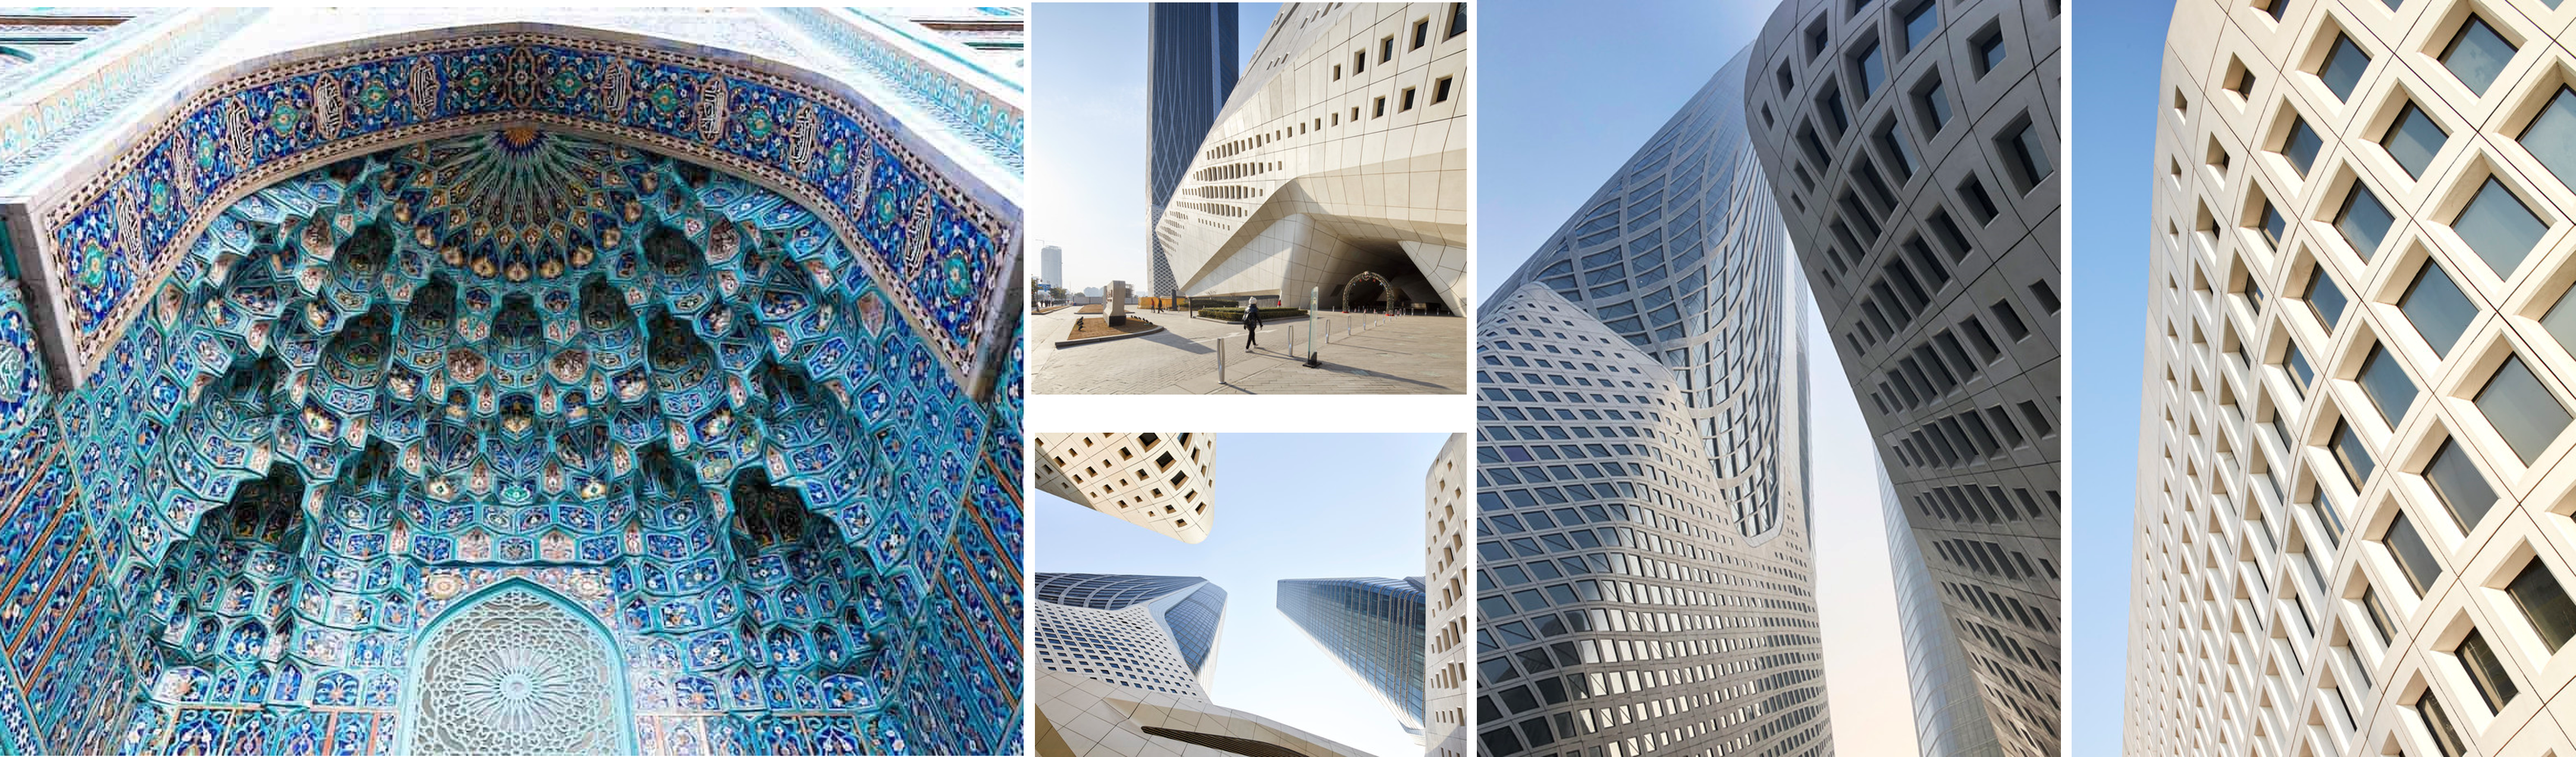
\includegraphics[width= \linewidth]{Images/complexornament}
          \caption{Complex ornament reference  (\textit{Images edited from source)}}
          \label{fig:complexornament}
        \end{figure*}



\section{Conclusions}
\label{sec:Conclusion}
%% The main conclusions of the study may be presented in a short Conclusions section, which may stand alone or form a subsection of a Discussion or Results and Discussion section.
%!%\section{Conclusions}
%%\label{sec:Conclusion}
%%%!%\section{Conclusions}
%%\label{sec:Conclusion}
%%%!%\section{Conclusions}
%%\label{sec:Conclusion}
%%\input{Text/Conclusions}

%% The main conclusions of the study may be presented in a short Conclusions section, which may stand alone or form a subsection of a Discussion or Results and Discussion section.
%% Answer the Research question

%revision

This research investigates architectural design at the intersection of digital fabrication, virtual reality (VR) assessment, and computer vision, aiming to deepen our understanding of complexity in facade design.
Our primary goal is to gauge user tolerance and acceptance of complex facades, offering insights into future construction practices.

A literature review confirmed that contemporary architecture is witnessing a trend towards increasing complexity in facade designs, moving away from the minimalist approach of the modernist movement, a trend also evidenced by the quantitative analysis across architectural history, provided by the `Computational Image Complexity Analysis' (CICA) system, which revealed an upward complexity trendline since the late 20th century (see Figure~\ref{fig:CICAscatterGraphRender}).
The historical analysis using the CICA system underscored the cultural and historical significance of facades, indicating that architectural complexity is not merely a matter of quantitative metrics but also involves cultural resonance and historical context.

Participants in the virtual reality experiment showed a preference for facades with moderate complexity, suggesting that future architectural trends may favor designs that balance intricacy with simplicity.
On average, participants favor a moderate level of complexity, with an average CICA complexity score of 3.82 (out of 10) and a 40\% probability of selecting a score close to this value according to CICA\@.

Discrepancies between participant perceptions and the CICA system's complexity rankings were particularly evident at higher complexity levels.
This highlights the subjective nature of complexity perception and the importance of integrating human feedback into architectural assessments.

The qualitative data suggests a shift towards customizable and user-responsive architectural solutions, with participants favoring form over materials and expressing a preference for facades that consider views and privacy.
This feedback suggests a strategic, view-dependent approach to facade complexity is crucial for user satisfaction.

In conclusion, this study underscores a shift in contemporary architecture towards embracing complexity in facade design, moving beyond the minimalist constraints of the modernist movement.
These insights could inform the development of nuanced and user-centric approaches in architectural design, catering to the evolving demands of modern society.


%% The main conclusions of the study may be presented in a short Conclusions section, which may stand alone or form a subsection of a Discussion or Results and Discussion section.
%% Answer the Research question

%revision

This research investigates architectural design at the intersection of digital fabrication, virtual reality (VR) assessment, and computer vision, aiming to deepen our understanding of complexity in facade design.
Our primary goal is to gauge user tolerance and acceptance of complex facades, offering insights into future construction practices.

A literature review confirmed that contemporary architecture is witnessing a trend towards increasing complexity in facade designs, moving away from the minimalist approach of the modernist movement, a trend also evidenced by the quantitative analysis across architectural history, provided by the `Computational Image Complexity Analysis' (CICA) system, which revealed an upward complexity trendline since the late 20th century (see Figure~\ref{fig:CICAscatterGraphRender}).
The historical analysis using the CICA system underscored the cultural and historical significance of facades, indicating that architectural complexity is not merely a matter of quantitative metrics but also involves cultural resonance and historical context.

Participants in the virtual reality experiment showed a preference for facades with moderate complexity, suggesting that future architectural trends may favor designs that balance intricacy with simplicity.
On average, participants favor a moderate level of complexity, with an average CICA complexity score of 3.82 (out of 10) and a 40\% probability of selecting a score close to this value according to CICA\@.

Discrepancies between participant perceptions and the CICA system's complexity rankings were particularly evident at higher complexity levels.
This highlights the subjective nature of complexity perception and the importance of integrating human feedback into architectural assessments.

The qualitative data suggests a shift towards customizable and user-responsive architectural solutions, with participants favoring form over materials and expressing a preference for facades that consider views and privacy.
This feedback suggests a strategic, view-dependent approach to facade complexity is crucial for user satisfaction.

In conclusion, this study underscores a shift in contemporary architecture towards embracing complexity in facade design, moving beyond the minimalist constraints of the modernist movement.
These insights could inform the development of nuanced and user-centric approaches in architectural design, catering to the evolving demands of modern society.


%% The main conclusions of the study may be presented in a short Conclusions section, which may stand alone or form a subsection of a Discussion or Results and Discussion section.
%% Answer the Research question

%Conclusion

This study investigates architectural design at the intersection of digital fabrication, VR assessment, and CV algorithms, aiming to deepen our understanding of complexity in facade design.
Our primary goal is to verify the practical application of a VR and CV based `Complexity Analysis' system for facade design, offering insights into user acceptance of complex facades.

A literature review theorized a current trend towards increasing complexity in contemporary architecture, moving away from the uniformity of barren walls and fully glazed facades approach of the modernist movement.
The CICA system quantitatively analyzed this same timeframe, proving this theory and revealing the existence of an upward complexity trendline since the late 20th century (see Figure~\ref{fig:CICAscatterGraphRender}).
Furthermore, the historical analysis using the CICA system underscored the cultural and historical significance of facades, indicating that architectural complexity is not merely a matter of quantitative metrics but also involves cultural resonance and historical context.

Participants in the experiment showed a preference for facades with moderate complexity, suggesting that future architectural trends may favor designs that balance intricacy with simplicity.
On average, participants preferred a moderate level of complexity, with a mean CICA complexity score of 4.05 (out of 10) and a 40\% probability of selecting a score close to this value.

Discrepancies between participant perceptions and the CICA system's complexity rankings, with an average standard deviation of 9\%,  were more evident at higher complexity levels, highlighting the subjective nature of complexity perception and the need to integrate human feedback into architectural assessments.
Qualitative data suggest a shift towards customizable and user-responsive architectural solutions, with participants favoring form over materials and preferring facades that consider views and privacy.

\textbf{Limitations}

While this research provides valuable insights into architectural complexity, certain limitations warrant cautious interpretation of the results:

%1 Sample Size and Demographic Representation:
\deleted{The study involved a relatively small sample of 26 participants, primarily university students and faculty members, which may limit the generalizability of the findings.}

\added{
The study involved a relatively small sample of 26 participants, primarily composed of university students, with 69.2\% aged between 18 and 24. Most participants lacked extensive professional experience in architecture, particularly in facade design. This limited demographic representation may affect the generalizability of the findings, as preferences for complexity could vary significantly with broader participant pools, including professionals with diverse levels of expertise and experience.
}

%2 Virtual Reality Environment:
The use of VR offered a controlled and immersive environment but may not entirely capture the experience of interacting with real-world facades.
VR settings could affect perceptions of complexity and comfort, leading to different results compared to real-world interactions.

%3 CICA System Metrics
The CICA system, while effective in evaluating architectural complexity using specific metrics, may not capture all elements influencing perceived complexity.
This underscores the need for further exploration of the subjective nature of complexity perception, which can be shaped by individual aesthetic preferences, prior experiences, and cultural factors, aspects that CV algorithms might struggle to fully capture.

%Image selection criteria and Historical Analysis Dataset:
\added{
 The evaluation is based on single images of each facade, which limits the ability to fully grasp the overall complexity of a building, as different perspectives might reveal additional elements that contribute to its perceived intricacy. This choice was made to standardize the analysis, but multiple images from different angles could provide a more comprehensive understanding of architectural complexity.}
The limited dataset of 177 historical buildings may restrict the comprehensiveness of the complexity assessment.
Expanding the dataset could yield a more detailed understanding of trends in architectural complexity over time.

%4 Focus on Facade Design
This study concentrated on facade design, which is just one aspect of architectural complexity.
CV models developed for specific architectural features might not generalize well to other styles or unique design elements, potentially limiting their applicability across diverse architectural contexts.
\added{
Furthermore, while the analysis provided valuable insights into surface-level details such as patterns and textures, the focus on facade-level complexity without addressing the overall volumetric complexity or massing of the building form implies that it lacks tools to capture the three-dimensional geometry that contributes to the holistic perception of architectural complexity. Future studies should incorporate assessments of volumetric complexity to provide a more comprehensive understanding of how building form influences user perception.
}

%%%%%%%%%%%%
\textbf{Limitations}

While this research provides valuable insights into architectural complexity, certain limitations warrant cautious interpretation of the results:

%1 Sample Size and Demographic Representation:
\deleted{The study involved a relatively small sample of 26 participants, primarily university students and faculty members, which may limit the generalizability of the findings.}

\added{
The study involved a relatively small sample of 26 participants, primarily composed of university students, with 69.2\% aged between 18 and 24. Most participants lacked extensive professional experience in architecture, particularly in facade design. This limited demographic representation may affect the generalizability of the findings, as preferences for complexity could vary significantly with broader participant pools, including professionals with diverse levels of expertise and experience.
}

%2 Virtual Reality Environment:
The use of VR offered a controlled and immersive environment but may not entirely capture the experience of interacting with real-world facades.
VR settings could affect perceptions of complexity and comfort, leading to different results compared to real-world interactions.

%3 CICA System Metrics
\deleted{The CICA system, while effective in evaluating architectural complexity using specific metrics, may not capture all elements influencing perceived complexity.
This underscores the need for further exploration of the subjective nature of complexity perception, which can be shaped by individual aesthetic preferences, prior experiences, and cultural factors, aspects that CV algorithms might struggle to fully capture.
}

\added{The CICA system, while effective in evaluating facade complexity using metrics like edge detection and contour count, may not capture all elements influencing perceived complexity. These metrics focus on two-dimensional visual data and might not fully address the subjective nature of complexity perception, which is shaped by individual aesthetic preferences, prior experiences, and cultural factors—factors that CV algorithms struggle to encapsulate. Furthermore, the system lacks tools to analyze three-dimensional articulation and hierarchical design elements, which are crucial to volumetric complexity and the overall form of buildings. This omission limits the system's ability to fully represent how buildings are perceived in terms of spatial interaction and three-dimensionality.
}

\added{
The survey questions focused mainly on surface-level details, such as patterns and textures, without addressing the building's overall form and three-dimensional geometry. Incorporating questions and metrics related to volumetric complexity would provide a more complete understanding of how architectural complexity is perceived in real-world settings.}

%Image selection criteria and Historical Analysis Dataset:
\deleted{
The limited dataset of 177 historical buildings may restrict the comprehensiveness of the complexity assessment.
Expanding the dataset could yield a more detailed understanding of trends in architectural complexity over time.
}
\added{
The evaluation in this study was based on single images of each facade, which, while necessary for standardization, may not fully represent the building's complexity as perceived from different angles. Using multiple images could reveal additional facets of architectural intricacy and provide a more robust complexity assessment. Additionally, the dataset of 177 historical buildings, while diverse, may limit the generalizability of trends in architectural complexity. Expanding this dataset to include more buildings from various eras and styles could offer a more detailed and representative understanding of complexity trends over time.
}

%4 Focus on Facade Design
This study concentrated on facade design, which is just one aspect of architectural complexity. \deleted{CV models developed for specific architectural features might not generalize well to other styles or unique design elements, potentially limiting their applicability across diverse architectural contexts}.
\added{
 While the insights into patterns, textures, and materials are valuable, the CV models developed for specific facade features might not generalize well to other architectural elements or styles.
}

%!%Highlight potential avenues for further research and development.

\textbf{Future Works}

The findings and limitations of this study provide opportunities for further exploration in architectural complexity:

%1Sample Size and Demographic Representation:
Future studies should involve a larger and more diverse group of participants to broaden the generalizability of the findings.
Conducting long-term studies could also shed light on the evolution of preferences for architectural complexity over time.

%2 Virtual Reality Environment:
Future research could compare VR-based assessments with evaluations of physical facades to better understand the correlation between virtual experiences and real-world perceptions.
Leveraging emerging technologies in Extended Reality (ER), such as Mixed Reality (MR) and Augmented Reality (AR), could further bridge the gap between virtual simulations and reality enhancing the assessment and prediction of user preferences in complexity in architectural design.

%3 CICA System Metrics and Historical Analysis Dataset:
\deleted{Future works could improve the accuracy of the CICA system by incorporating additional metrics, such as color, texture, and contextual integration.}

\added{
Future works could improve the accuracy of the CICA system by incorporating additional metrics such as color, texture, and contextual integration, providing a more nuanced understanding of facade complexity. In particular, incorporating volumetric complexity, such as the three-dimensional articulation, massing, and hierarchical design elements, would significantly enhance the system’s ability to capture how buildings are perceived holistically in real-life contexts. This could be achieved by developing tools that assess not just the surface-level details but also the overall building form and its spatial interaction with the environment.}
Developing methodologies that integrate user feedback more directly into the design process could lead to more personalized and culturally sensitive architectural solutions.
Future iterations should consider both the quantitative aspects of facade complexity and the cultural resonance and historical context to provide a comprehensive evaluation of architectural evolution.

%4 Focus on Facade Design
Furthermore, future research should encompass additional elements, such as interior design and spatial organization, to achieve a more holistic understanding of architectural complexity.
\deleted{Examining the relationship between architectural complexity and sustainability could also provide insights into how complex designs can contribute to or detract from sustainable building practices.}
\added{Investigating the relationship between architectural complexity and sustainability could also provide insights into how complex designs impact sustainable building practices, helping architects balance intricate aesthetics with environmental considerations.}

%%Closing statement
In conclusion, this study successfully addressed the challenge of quantifying complexity in architectural facade design through the integration of VR and CV technologies.
Furthermore, it also provides valuable insights into user preferences, thereby has the potential of enhancing DBD processes.
This can prove useful for guiding the optimization of building design towards a more user-centric approach in architectural design, catering to the evolving demands of modern society.



\section{Declaration of Competing Interest}
\label{sec:DeclarationInterest}
%% Declaration of using AI to edit the text
\input{Text/DeclarationInterests}

%\section{Declaration of generative AI and AI-assisted technologies in the writing process}
%\label{sec:Declaration AI}
%% Declaration of using AI to edit the text
%%%Declaration of generative AI and AI-assisted technologies in the writing process

During the preparation of this work, the author(s) used CHAT GPT/ OPEN AI in order to improve language and readability.
After using this tool/service, the author(s) reviewed and edited the content as needed and take(s) full responsibility for the content of the publication.

%% End of line numbers
\end{linenumbers}

%% If you have bibdatabase file and want bibtex to generate the
%% bibitems, please use
%%
%\newpage
%\clearpage
\bibliographystyle{elsarticle-num}
\bibliography{main}

%% The Appendices part is started with the command \appendix;
%% appendix sections are then done as normal sections
%\newpage
%\clearpage
\appendix

\section{3D-modeled Facade Variations across Patterns}
\label{sec:AnnexVariations}
\input{Text/AnnexVariations}

\end{document}